\documentclass[12pt,oneside]{book}

\usepackage{latexsym}
\usepackage[empty]{fullpage}
\usepackage{titlesec}
\usepackage{marvosym}
\usepackage[usenames,dvipsnames]{color}
\usepackage{verbatim}
\usepackage{enumitem}
\usepackage{etoolbox}

\usepackage{xcolor}
\usepackage{times}
\usepackage{lastpage}

\renewcommand\bibname{ }
%\usepackage{mathptmx}
\usepackage{graphicx}
\usepackage{wrapfig}
\usepackage[utf8]{inputenc}
\usepackage{fancyhdr}
 \pagestyle{fancy}
\fancyhf{}
%\lhead{Curriculum vitae}
\cfoot{ \hrule {\small Moslem Heidarpur}{\hfill\small Page \thepage ~of  \pageref{LastPage}}}
 \usepackage{geometry}
 \geometry{
 a4paper,
 total={170mm,257mm},
 left=15mm,
 top=17mm,
 right=15mm,
  bottom=37mm,
 }
\setlength{\headsep}{0.2in} 
\setlength{\footskip}{0.5in} 

\newcommand{\fd}{\small \textit}
%\newcommand{\mtf}{ \fontfamily{put}\selectfont}
\newcommand{\mtf}{ \bf \normalsize}
\usepackage{array}
\newcolumntype{L}[1]{>{\raggedright\let\newline\\\arraybackslash\hspace{0pt}}m{#1}}
\newcolumntype{C}[1]{>{\centering\let\newline\\\arraybackslash\hspace{0pt}}m{#1}}
\newcolumntype{R}[1]{>{\raggedleft\let\newline\\\arraybackslash\hspace{0pt}}m{#1}}

\usepackage[resetlabels]{multibib}
\bibliographystyle{ieeetr}
%\newcites{crypto}{{dff}} 
\definecolor{darkgreen}{rgb}{0,0.5,0}
\patchcmd{\thebibliography}{\chapter*}{\section*}{}{}
\renewcommand{\headrule}{{\color{gray}\hrule width\headwidth height\headrulewidth \vskip-\headrulewidth}}
\newcites{main,crypto}{{},{}}

\usepackage{hyperref}
\hypersetup{
    colorlinks=true,
    linkcolor=black,  % color of internal links
    urlcolor=blue    % color of external links
}
\newcommand{\position}{Sessional Assistant Professor, Teaching Stream (Software Development) }
\newcommand{\department}{Department of Electrical Engineering and Computer Science}
\newcommand{\university}{York University}
\begin{document}\thispagestyle{empty}
\vspace*{-5em} \phantom \quad \\
\today\\
%\vspace*{0\baselineskip}\phantom \quad \\
Chair, Faculty Search Committee\\
\department ,\\
\university ,\\
204 Bergeron Centre, \\
North York, ON, M3J 2S5.\\
%\vspace*{2\baselineskip}
\phantom \quad \\
Dear Hiring Committee,\\

I am writing to express my interest in the \position ~position   \department at \university. Throughout my professional journey, I have gained diverse teaching experiences. 

I taught at a vocational high school for two years and served as a seasonal lecturer at Islamic Azad University, Iran, instructing courses in computer architecture and digital logic design. Additionally, during my PhD, I played an active role in teaching and preparing course materials for subjects such as Digital Logic Design, Embedded Systems, and Electronics. As a postdoctoral fellow and part-time researcher at the University of Windsor, I provided guidance to PhD, MSc, and bachelor students. In my capacity as a seasonal instructor for continuing education, I conducted online courses in Cybersecurity.

In my industry experience as a Logic Design Engineer at NXP Semiconductors, I was responsible for designing high-performance network controllers for Ethernet switches. This role involved reading frame data from memory, performing frame modifications, ensuring frame integrity, and implementing functional safety mechanisms. As an SOC Design Engineer at Axiado, I contributed to designing various System On Chips (SOCs), including one utilizing ARM CPUs with Cortex A53, Cortex M55, Cortex M0, and Ethos U65 for artificial neural networks in cybersecurity applications.

My research focus has been in neuromorphic engineering, post-quantum, and homomorphic encryption circuit and systems. During my MSc and PhD, I developed novel techniques to enhance the performance and reduce the area of systems implementing Spiking Neural Networks (SNNs). These networks, being the third generation of neural networks, offer significant advantages for classification and medical purposes. In my postdoctoral role, I initiated research on simplifying complexity and designing hardware for low-latency and low-area finite field multipliers used in cryptosystems. As a part-time research assistant at the University of Windsor, my work involves designing efficient hardware architectures for implementing Post-Quantum Cryptography (PQC) and Homomorphic Encryption (HE) systems, resulting in  journal publications,  conference papers, and  U.S. patents.

Having been inspired by exceptional teachers and advisers, I recognize the profound impact a dedicated educator can have on a student. I am committed to following in their footsteps, continually improving my teaching and research skills.

Thank you for considering my application.
\vspace*{1\baselineskip}
\phantom \quad \\
Sincerely,\\[0.2cm]
%\vspace*{1\baselineskip}
%\phantom \quad \\
Moslem Heidarpur\\
217 Big Dipper St., Ottawa, ON, Canada, K4M 0J8\\
Email: heidarpur.m@gmail.com\\
Immigration status: Permanent resident of Canada\\[-0.1cm]
\newpage
\lhead{\textcolor{gray}{Curriculum vitae}}
\large \bf \hphantom \\ \\ 
 {\fontfamily{put}\selectfont Moslem Heidarpur} \mdseries \normalsize \\ \\ 
 \begin {itemize}
\item [] \phantom \quad  \item   []  {\bf  Webpages:} \vspace{-1.5em}
\item []  {\bf \hrulefill } \vspace{-1em}
\begin {itemize}
\item  \small \href{https://orcid.org/0000-0002-4116-0778 } {ORCID} 
%\item ORCID: \begin {itemize}  \item[] https://orcid.org/0000-0002-4116-0778 (\href{https://orcid.org/0000-0002-4116-0778 } {Hyperlink})  
%\end {itemize} 
%\item Google Scholar: \begin {itemize}  \item[] https://scholar.google.com/citations?user=bVzQEKkAAAAJ$\&$hl=en$\&$oi=ao  
\item \small \href{https://scholar.google.com/citations?user=bVzQEKkAAAAJ&hl=en&oi=ao  } { Google Scholar}
%\end {itemize}
%\item Linkedin:\begin {itemize}  \item[] https://www.linkedin.com/in/moslemheidarpur/ 
\item \small \href{https://www.linkedin.com/in/moslemheidarpur/   } {Linkedin}
 %\end {itemize}
%\item Researchgate:\begin {itemize}  \item[]  https://www.researchgate.net/profile/Moslem-Heidarpur 
\item \small \href{ https://www.researchgate.net/profile/Moslem-Heidarpur   } {Researchgate}
% \end {itemize}
\end{itemize}  \vspace{0.5em}
\item  []  {\bf  Immigration status:}  \vspace{-1.5em}
\item []  {\bf \hrulefill } \vspace{-1em}
\begin {itemize} \item \small Permanent resident of Canada
\end {itemize}   \vspace{0.5em}
\item  [] {\bf  Address:} \vspace{-1.5em}
\item []  {\bf \hrulefill } \vspace{-1em}
\begin {itemize} 
\item  \small 217 Big Dipper, Ottawa, ON, Canada
\end{itemize}  \vspace{0.5em}
\item  []  {\bf  Email:} \vspace{-1.5em}
\item []  {\bf \hrulefill } \vspace{-1em}
\begin {itemize} 
 \item  \small heidarpur.m@gmail.com (preferred)
 \item \small heidarp@uwindsor.ca
 \item \small moslem.heidarpur@nxp.com
\end {itemize}   \vspace{0.5em}
\item  []   {\bf Phone:} \vspace{-1.5em}
\item []  {\bf \hrulefill } \vspace{-1em}
\begin {itemize} 
\item 613-797-6194
\end{itemize}
\end{itemize}

\newpage
\begin {itemize} \item [] {\bf \Large  Education }  \vspace{-1.5em}
\item []  {\bf \hrulefill } 
\mdseries \normalsize 
\begin {itemize}
\item [$\bullet$] \bf {\mtf \normalsize PhD in Electrical Engineering} \mdseries
    \begin {itemize}
        \item [-]  {   University:} 
          \small University of Windsor, ON, Canada.\small \hspace{3.8cm}\textit{2020}\normalsize
        \item [-]   {   Dissertation Title:} 
               Digital Implementation and Modification: Spiking Neural Network
        \item [-]  {   Dissertation Advisors:} 
                Majid Ahmadi, Distinguished Professor, 
              Arash Ahmadi, Assistant Professor.
    \end {itemize} \vspace{0.3cm}
\item [$\bullet$]  \bf {\mtf \normalsize  M.Sc. in Electrical Engineering } \mdseries
    \begin {itemize}
        \item [-]  {   University:} 
          Razi University of Kermanshah, Kermanshah, Iran.\small \hspace{0.85cm}\textit{2014}\normalsize
        \item [-]   {   Dissertation Title:} 
               Digital Implementation of a concise model for astrocyte calcium oscillations.
        \item [-]  {   Dissertation Advisors:} 
                Arash Ahmadi, Assistant Professor
    \end {itemize}\vspace{0.3cm}
\item [$\bullet$] \bf {\mtf  \normalsize B.Sc. in Electrical Engineering} \mdseries
    \begin {itemize}
    \item [-] {University:} {\small Razi University of Kermanshah, Kermanshah, Iran}\small  \hspace{1.6cm} \textit{2009}\normalsize 
    \item [-]   {   Project Title:} 
               Digital Implementation of a PC Oscilloscope
        \item [-]  {   Project Advisors:} 
                Mohsen Hayati, Professor
    \end {itemize}
\end {itemize} \vspace{1cm}
\item [] {\bf \Large  Industry Training and Courses }   \vspace{-1.5em}
\item []  {\bf \hrulefill } 
\begin {itemize}
    \item [$\bullet$] \bf {\mtf \normalsize Functional Safety} \mdseries
        \begin {itemize}
            \item [-] Introduction to functional safety, why it is required, and its implications
            \item [-] Meeting requirements of ISO26262 and IEC 61508
        \end {itemize} \vspace{0.3cm}
    \item [$\bullet$] \bf {\mtf \normalsize Design Excellence and Quality Management System (QMS) } \mdseries    
        \begin {itemize}
             \item [-] Documenting policies, procedures and controls necessary to create high-quality products
            \item [-] Meeting requirements of ISO 9001 and IATF 16946
        \end {itemize}\vspace{0.3cm}
       \item [$\bullet$] \bf {\mtf \normalsize Root Cause Analysis (RCA) } \mdseries
         \begin {itemize}
            \item [-] 8-D (8-Discipline) problem solving process
            \item [-] 3x5 why analysis and  Corrective Action (CA)
        \end {itemize} \vspace{0.3cm}
       \item [$\bullet$] \bf {\mtf \normalsize Cross Domain Clocking (CDC)  } \mdseries
         \begin {itemize}
            \item [-] Historical issues related to CDC mishandling leading to Mean Time between Failures (MTBF) 
            \item [-] Best approaches to asynchronous communication between modulus running on different clock frequencies
        \end {itemize}\vspace{0.3cm}
       \item [$\bullet$] \bf {\mtf \normalsize Right Review Training  } \mdseries
         \begin {itemize}
            \item [-] Right Reviews (Review of code, documentation, specification etc. ) and characteristics 
            \item [-] Roles and Responsibilities recommended to conduct review and validation process 
        \end {itemize}\vspace{0.3cm}
       \item [$\bullet$] \bf {\mtf \normalsize Practical development of risk management for process  } \mdseries
         \begin {itemize}
            \item [-] Introduction to risk management, process steps, and roles and responsibilities
            \item [-] Change management system and  risk register
        \end {itemize}\vspace{0.3cm}
            \item [$\bullet$] \bf {\mtf \normalsize Business Creation and Management (BCaM) } \mdseries
         \begin {itemize}
            \item [-] R$\&$D policies at the corporation
            \item [-] Design Failure Modes and Effects Analysis (DFMEA)
        \end {itemize}\vspace{0.3cm}
\end {itemize}
\end {itemize}
 
\newpage

\begin {itemize} \item [] {\bf \Large   Teaching Experience }  \vspace{-1.5em}
\item []  {\bf \hrulefill } \mdseries \normalsize 
    \begin {itemize}
        \item [$\bullet$] \bf {\mtf \normalsize  Instructor,  University of Windsor} \mdseries
            \begin {itemize}
                \item [-]  {  Location: Continuing Education, Windsor, ON, Canada.\small \hspace{2.1cm}\textit{2023-Present}\normalsize} 
                \item [-]   {   Description:} 
                    \begin {itemize}   
                        \item [\textbullet] Courses are offered remotely, where students learn about different types of cyber attacks and how to secure computers, networks, and servers
                        \item [\textbullet] Course materials, attendance, quizzes, and grading were online in Brightspace.
                    \end {itemize}
                    \item [-]   {   Courses:} 
                    \begin {itemize}   
                        \item [\textbullet]  Cybersecurity I : Introduction to Systems Security 
                        \item [\textbullet] Cybersecurity II: System Implementation
                    \end {itemize}
            \end {itemize} \vspace{0.3cm}
    %--------------------------------
     \item [$\bullet$] \bf {\mtf \normalsize Mentor, University of Windsor} \mdseries
            \begin {itemize}
                \item [-]  {  Location:  Windsor, ON, Canada\small \hspace{5.8cm}\textit{2020-Present}\normalsize} 
                \item [-]   {   Description:} 
                    \begin {itemize}
                        \item [\textbullet] Closely supervising and mentoring four PhD and seven master students on weekly meeting basis.
                        \item [\textbullet] Helping them to gain fundamental knowledge, identifying problems, literature survey for solutions, and critical analysis of published works.
                        \item [\textbullet] PhD students have successfully published papers in IEEE transactions within their second year, with additional papers currently under review and in preparation
                        \item [\textbullet] Offered guidance and evaluate the progress of an undergraduate student as they completed their project.
                    \end {itemize}
            \end {itemize} \vspace{0.3cm}
%--------------------------------
     \item [$\bullet$] \bf {\mtf \normalsize  Graduate Teaching Assistant, University of Windsor} \mdseries
            \begin {itemize}
                \item [-]  {  Location: Windsor, ON, Canada.\small \hspace{5.7cm}\textit{2019-2020}\normalsize} 
                \item [-]   {   Description:} 
                    \begin {itemize}
                        \item [\textbullet]  Prepared materials, tutorials and answered student questions as a teaching assistant
                        \item [\textbullet]  During  labs, I 
helped students to formulate their ideas to flowcharts and further to codes to implement on FPGA, Arduino or Raspberry Pi evaluation boards
 and eventually debugging it.
                    \end {itemize}
                    \item [-]   {   Courses:} 
                    \begin {itemize}   
                        \item [\textbullet]  Digital Logic Design II
                        \item [\textbullet] Embedded Systems
                        \item [\textbullet] Electronics I
                    \end {itemize}
            \end {itemize} \vspace{0.3cm}         
%--------------------------------
     \item [$\bullet$] \bf {\mtf \normalsize   Lecturer, Islamic Azad University} \mdseries
            \begin {itemize}
                \item [-]  {  Eslamabad-Gharb, Kermanshah, Iran\small \hspace{5cm}\textit{2018-2020}\normalsize} 
                \item [-]   {  Description:} 
                    \begin {itemize}
                        \item [\textbullet]  Delivered lectures, designed, prepared, and developed teaching materials, and assessed students.
                        \item [\textbullet]  Supervised  final year undergraduate projects.
                    \end {itemize}
                    \item [-]   {   Courses:} 
                    \begin {itemize}   
                        \item [\textbullet] Digital Logic Design
                        \item [\textbullet]  Computer Architecture
                        \item [\textbullet] Analog CMOS Integrated Circuits
                         \item [\textbullet] Electronics
                    \end {itemize}    
            \end {itemize} \vspace{0.3cm}   
%--------------------------------
     \item [$\bullet$] \bf {\mtf \normalsize   High School Teacher, Chamran Vocational High School} \mdseries
            \begin {itemize}
                \item [-]  {  Eslamabad-Gharb, Kermanshah, Iran\small \hspace{5cm}\textit{2010-2012}\normalsize} 
                \item [-]   { Description:} 
                    \begin {itemize}
                        \item [\textbullet]  Taught Courses in school and evaluated students
                        \item [\textbullet]  Worked  with weaker students in individual
                        \item [\textbullet]  Graded  exams and communicated with parents about students progress.
                    \end {itemize}
                     \item [-]   {   Courses:} 
                    \begin {itemize}   
                        \item [\textbullet]  Electronics Measurements
                         \item [\textbullet] Electronics
                    \end {itemize}    
            \end {itemize} \vspace{0.3cm}   
    \end {itemize}
\end {itemize}











% \end{minipage} \phantom  \mdseries \\ [0.2cm]
%\begin{tabular}{L{14cm}p{1cm}r} \bf  { Graduate Teaching Assistant, University of Windsor, ON, Canada. }&&\mdseries \fd{2018-2020}\mdseries  \normalsize  \end{tabular} \\
%\phantom \quad $\bullet$ \begin{minipage}[t]{0.965\textwidth}  Prepared materials, tutorials and answered student questions as a teaching assistant. During  labs, I 
%helped students to formulate their ideas to flowcharts and further to codes to implement on FPGA, Arduino or Raspberry Pi evaluation boards
% and eventually debugging it.   \\[0.1cm]
% Courses: Digital Logic Design II (DLDII), Embedded Systems and Electronics I
%\end{minipage}\\ [0.2cm]
%\begin{tabular}{L{12cm}p{3cm}r} \bf  {  Lecturer, Islamic Azad University,  Kermanshah, Iran.} &&\mdseries\fd{2014-2018}\mdseries  \normalsize \end{tabular}\\
%\phantom \quad $\bullet$ \begin{minipage}[t]{0.965\textwidth}  
%Delivered lectures, designed, prepared and developed courses and teaching materials and assessed students. Supervised  research activities of students  including final year undergraduate projects.\\ [0.2cm]
%Courses: Digital Logic Design, Computer Architecture and Analog CMOS Integrated Circuits, Electronics. 
% \end{minipage} \phantom  \mdseries 
% \\ [0.2cm]
% \begin{tabular}{L{14cm}p{1cm}r} \bf  {  High School Teacher, Chamran High School,  Eslamabad Gharb, Iran.} &&\mdseries\fd{2009-2010}\mdseries  \normalsize \end{tabular}\\
%\phantom \quad $\bullet$ \begin{minipage}[t]{0.965\textwidth}  
%Designed courses, instructed and evaluated students, worked  with weaker students in individual,  graded  exams and communicated with parents about students progress.\\ [0.2cm]
%Courses: Electronics, Electronics Measurements. 
% \end{minipage} \phantom  \mdseries \\ \\

\newpage


\begin {itemize} \item [] {\bf \Large   Academic Services }  \vspace{-1.5em}
\item []  {\bf \hrulefill } \mdseries \normalsize 
    \begin {itemize}
        \item [$\bullet$] \bf {\mtf \normalsize  Guest Reviewer To  Journals and Conferences.} \mdseries
        \item [-]   {   Description:} 
        \begin {itemize}
                        \item [\textbullet] Conducted peer review of papers for possible publication in the  journals and conferences
                    \end {itemize}
            \begin {itemize}
                \item [-]   {   Journals and Conferences:} 
                    \begin {itemize}   
                        \item [\textbullet]  IEEE Transactions on Circuits and Systems  I (TCAS I)
                        \item [\textbullet] IEEE Transactions on Very Large Scale Integration (VLSI) Systems (TVLSI) 
                         \item [\textbullet] IEEE Transactions on Biomedical Circuits and Systems (TBIOCAS)
                          \item [\textbullet] Neural Computing and Applications
                           \item [\textbullet] IEEE Access
                            \item [\textbullet] Microelectronics Journal
                            \item [\textbullet] IEEE Transactions on Emerging Topics in Computational Intelligence (TETCI) 
                             \item [\textbullet] IEEE International Symposium on Circuits and Systems (ISCAS)
                    \end {itemize}
            \end {itemize} \vspace{0.3cm}
    %--------------------------------
     \item [$\bullet$] \bf {\mtf \normalsize Review Committee Members (RCM)} \mdseries
            \begin {itemize}
                \item [-]   {   Description:} 
                    \begin {itemize}
                        \item [\textbullet] Assigned reviewers to papers and follow up regarding reviews
                         \item [\textbullet] Preliminary decision on papers based on reviewer comments
                    \end {itemize}
                        \item [-]   {   Journals and Conferences:} 
                    \begin {itemize}   
                        \item [\textbullet] IEEE International Symposium on Circuits and Systems (ISCAS) 2024 
                        \item [\textbullet] IEEE International Symposium on Circuits and Systems (ISCAS) 2023
                    \end {itemize}
            \end {itemize} \vspace{0.3cm}
%--------------------------------
     \item [$\bullet$] \bf {\mtf \normalsize  Vice Chair of IEEE Signal Processing Societies} \mdseries
            \begin {itemize}
                \item [-]  {  Location: Windsor, ON, Canada.}
                \item [-]   {   Description:} 
                    \begin {itemize}
                        \item [\textbullet]  Organized events, workshops and tutorials  as well as running  face-to-face meeting and performing chair duties in his absence.
                        \item [\textbullet] Presented a workshop on spiking neural networks and their application in signal processing. 
                    \end {itemize}
            \end {itemize} \vspace{0.3cm}         
    \end {itemize}
\end {itemize}















%{\bf  Other Relevant Experiences  }\hrulefill \\ \\ \mdseries \normalsize
%\begin{tabular}{L{12cm}p{3cm}r}\bf  {Digital Logic Designer, NXP Semiconductors, ON, Canada.}&&\mdseries \fd {2021-present } \end{tabular}\normalsize \mdseries\\
% \phantom \quad $\bullet$ \begin{minipage}[t]{0.965\textwidth} 
% Responsible for designing high performance network controllers for Ethernet switches. The designed unit is capable of receiving, modifying, storing and sending Ethernet frames using innovative techniques. Simulation are performed to ensure validity  of design. Further, the designed unit is synthesized to study performance and resources. If necessary, it may be modified again to meet the criteria.  
% \end{minipage}  
% \mdseries\\  \\
%\begin{tabular}{L{12cm}p{3cm}r}\bf  { System On Chip Engineer, Axiado Canada, ON, Canada.}&&\mdseries \fd {2021-2021 } \end{tabular}\normalsize \mdseries\\
% \phantom \quad $\bullet$ \begin{minipage}[t]{0.965\textwidth} 
%Designed system on chip using ARM CPUs including Cortex A53, Cortex M55, Cortex M0, Ethos U65, AXI interconnect etc. HDL Programming (System Verilog, Verilog). Computer architecture design, simulation  and performance monitoring.  Writing tests and programs using Bare Metal C. \end{minipage}  
% \mdseries\\  \\
% \begin{tabular}{L{12cm}p{3cm}r}\bf  { Vice Chair of IEEE Signal Processing Societies, ON, Canada.}&&\mdseries \fd {2018-Present } \end{tabular}\normalsize \mdseries\\
% \phantom \quad $\bullet$ \begin{minipage}[t]{0.965\textwidth} 
%Organized events, workshops and tutorials  as well as running  face-to-face meeting and performing chair duties in his absence.
%In addition, presented a workshop on spiking neural networks and their application in signal processing. \end{minipage}  
% \mdseries\\  \\
%\begin{tabular}{L{12cm}p{3cm}r}\bf \bf  { Guest Reviewer To  Journals and Conferences.} &&\mdseries \fd {2014-Present } \end{tabular}\normalsize \mdseries\\
% \phantom \quad $\bullet$     \begin{minipage}[t]{0.965\textwidth}
%  Conducted peer review of papers for possible publication in the  journals and conferences including: IEEE Transactions on Circuits and Systems  I (TCAS I), IEEE Transactions on Circuits and Systems  II (TCAS II), IEEE Transactions on Very Large Scale Integration (VLSI) Systems (TVLSI), IEEE Transactions on Biomedical Circuits and Systems (TBIOCAS),  Neural Computing and Applications, IEEE access, Microelectronics Journal, IEEE International Symposium on Circuits and Systems (ISCAS) etc.\end{minipage} \phantom  \mdseries \\ 
%\begin{tabular}{L{12cm}p{3cm}r}\bf  { Android Developer, Self-employed }&&\mdseries \fd{ 2018-Present }\mdseries \normalsize \end{tabular}\\
%\phantom \quad $\bullet$  \begin{minipage}[t]{0.965\textwidth} Active google play developer with more than 12000 active app installations.
% These apps include dictionaries, nomenclatures and classic poems which were developed in Eclipse and Android studio IDEs. 
%\end{minipage}\\  \\ \\

\newpage
\begin {itemize} \item [] {\bf \Large   Work Experience }  \vspace{-1.5em}
\item []  {\bf \hrulefill } \mdseries \normalsize 
    \begin {itemize}
    \item [$\bullet$] \bf {\mtf \normalsize  ASIC Design Engineer, Synopsys} \mdseries
            \begin {itemize}
                \item [-]  {  Location:  Ottawa, ON,  Canada.\small \hspace{5.8cm}\textit{2024-Present}\normalsize} 
                \item [-]   {   Job Description:} 
                    \begin {itemize}   
                        \item [\textbullet] Conducting research and development to improve DDR PHY performance and reliability.
                        \item [\textbullet] Assisting customers with questions related to PHY design and integration
                        \item [\textbullet] Developed an AI-based IP setting inspection and optimization tool (ISIO) to detect incorrect settings and optimize PHY eye quality.
                        \item [\textbullet] Added new features and extended the RDS tool to enhance debugging capabilities for customer issues.
                    \end {itemize}
            \end {itemize} \vspace{0.3cm}
        \item [$\bullet$] \bf {\mtf \normalsize  Digital Logic Designer, NXP Semiconductors} \mdseries
            \begin {itemize}
                \item [-]  {  Location:  Ottawa, ON,  Canada.\small \hspace{5.8cm}\textit{2021-2024}\normalsize} 
                \item [-]   {   Job Description:} 
                    \begin {itemize}   
                        \item [\textbullet] Responsible for designing high performance network controllers for Ethernet switches.
                        \item [\textbullet] The designed unit decoded the frame descriptor, extracted pointers and performed memory reads.
                        \item [\textbullet] ECC check block was coded to ensure the integrity of received data
                        \item [\textbullet] block was designed to decode and perform frame modification instructions received with frame context
                        \item [\textbullet] Parity check and fault injection and detection mechanism was coded for
safety enabled SOCs.
                    \end {itemize}
            \end {itemize} \vspace{0.3cm}
    %--------------------------------
     \item [$\bullet$] \bf {\mtf \normalsize  System On Chip Engineer, Axiado Canada} \mdseries
            \begin {itemize}
                \item [-]  {  Location:  Ottawa, ON,  Canada.\small \hspace{5.8cm}\textit{2020-2021}\normalsize} 
                \item [-]   {   Job Description:} 
                    \begin {itemize}
                        \item [\textbullet] Designed system on chip using ARM CPUs including Cortex A53, Cortex M55, Cortex M0, Ethos U65, AXI interconnect etc. 
                        \item [\textbullet] HDL Programming (System Verilog, Verilog), architecture, simulation  and performance monitoring.  
                        \item [\textbullet] Writing basic tests and programs using Bare Metal C. 
                        \item [\textbullet] The objective was to design an SOC that could inspect the Ethernet packets and detect cyber threats
using A
                    \end {itemize}
            \end {itemize} \vspace{0.3cm}
%--------------------------------
     \item [$\bullet$] \bf {\mtf \normalsize  Postdoctoral Researcher, University of Windsor} \mdseries
            \begin {itemize}
                \item [-]  {  Location: Windsor, ON, Canada.\small \hspace{5.5cm}\textit{2019-2020}\normalsize} 
                \item [-]   {   Job Description:} 
                    \begin {itemize}
                        \item [\textbullet]  Closely supervising and mentoring two PhD students and coordinating their research.
                        \item [\textbullet]  Identification of funding opportunities and writing of funding applications. 
                    \end {itemize}
            \end {itemize} \vspace{0.3cm}         
%--------------------------------
     \item [$\bullet$] \bf {\mtf \normalsize   Android Developer, Freelance} \mdseries
            \begin {itemize}
                \item [-]  {  Freelance.\small \hspace{9.2cm}\textit{2018-present}\normalsize} 
                \item [-]   {   Job Description:} 
                    \begin {itemize}
                        \item [\textbullet]  Google play developer with more than 12000 active app installations
                        \item [\textbullet]  apps include dictionaries, nomenclatures and classic poems which were developed in Eclipse and Android studio IDEs (Based on Java)
                    \end {itemize}
            \end {itemize} \vspace{0.3cm}    
    \end {itemize}
\end {itemize}


\newpage
\begin {itemize} 
    \item [] {\bf \Large  Technical Skills  }  \vspace{-1.5em}
    \item []  {\bf \hrulefill } \mdseries \normalsize 
        \begin {itemize}
            \item [$\bullet$] \bf {\mtf \normalsize  HDL} \mdseries
                    \begin {itemize}
                        \item [-] System Verilog
                        \item [-] Verilog
                        \item [-] VHDL
                    \end {itemize}
              \item [$\bullet$] \bf {\mtf \normalsize  Programming} \mdseries
                    \begin {itemize}
                        \item [-] Python
                        \item [-] C++
                        \item [-] Bare Metal C
                        \item [-] Java
                        \item [-] Assembly
                        \item [-] Latex
                        \item [-] Linux Shell Scripting
                    \end {itemize} 
               \item [$\bullet$] \bf {\mtf \normalsize  AI} \mdseries 
                    \begin {itemize}
                            \item [-] Neural Network
                            \item [-] Deep Learning
                            \item [-] Spike Time Dependent Plasticity (STDP)
                    \end {itemize} 
               \item [$\bullet$] \bf {\mtf \normalsize  CPUs and microcontrollers} \mdseries 
                     \begin {itemize}
                            \item [-] Cortex M55
                            \item [-] Cortex A53
                            \item [-] Cortex M0
                            \item [-] Ethos U65
                            \item [-] Zilog Z80
                            \item [-] Arduino
                            \item [-] Raspberry Pi.
                            \item [-] 8051 Microcontroller
                            \item [-] AXI Interconnect
                    \end {itemize} 
               \item [$\bullet$] \bf {\mtf \normalsize  Optimization} \mdseries 
                     \begin {itemize}
                            \item [-] Single and multi objective Particle Swarm  Optimization (PSO)
                            \item [-] Genetic Algorithm
                    \end {itemize} 
               \item [$\bullet$] \bf {\mtf \normalsize  Software and Tools} \mdseries 
                      \begin {itemize}
                            \item [-] Synopsys VCS
                            \item [-] Synopsys Lint
                            \item [-] Synopsys SpyGlass
                            \item [-] Siemens PowerPro
                            \item [-] Siemens Questa
                            \item [-] Cadence Genus Synthesis
                            \item [-] Verplex's BlackTie
                            \item [-] Xilinx ISE
                            \item [-] Xilinx Vivado
                            \item [-] Quartus prime
                            \item [-] Modelsim
                            \item [-] Matlab
                            \item [-] Hspice
                            \item [-] Agilent Advanced Design System
                            \item [-] Microsoft Visual Studio
                            \item [-] Eclipse
                            \item [-] Android Studio
                            \item [-] DesignSync
                            \item [-] Git
                            \item [-] Jira
                    \end {itemize} 
         \end {itemize}      
\end {itemize} 




%\bf\large  {\fontfamily{put}\selectfont Technical Skills } \hrulefill \\ \\ \mdseries \normalsize
%%\begin{tabular}{p{0.25\textwidth}p{.25\textwidth}
%\begin{tabular}{lp{13.2cm}}
%\bf  {\fontfamily{put}\selectfont HDL:}&   \mdseries  Digital hardware design using VHDL and Verilog.\\
%\bf  {\fontfamily{put}\selectfont Programming: }& \mdseries C++, Java, Assembly, Latex, Familiar with  Linux Shell Scripting and HTML. \\
%\bf  {\fontfamily{put}\selectfont Neural Networks:}&  \mdseries {\fontfamily{lmr}\selectfont Deep Learning and Spike Time Dependent Plasticity (STDP).}\\
%\bf  {\fontfamily{put}\selectfont RFIC:}& \mdseries Low noise amplifiers (LNA) design.\\
%\bf  {\fontfamily{put}\selectfont Optimization:} &  \mdseries   Single and multi objective Particle Swarm  Optimization (PSO).\\
%\bf  {\fontfamily{put}\selectfont Microcontrollers: }& \mdseries Experience with Zilog Z80, 8051 Microcontroller, Arduino and Raspberry Pi.\\ 
%\bf  {\fontfamily{put}\selectfont Software: }& \mdseries  Matlab, Xilinx ISE, Quartus prime, Cadence, Synopsys, Modelsim, Agilent Advanced Design System, Hspice, 
% Microsoft Visual Studio, Eclipse, Android Studio.\\
%\end{tabular} \\ \\ 

\newpage

\begin {itemize} \item [] {\bf \Large   Grants }  \vspace{-1.5em}
\item []  {\bf \hrulefill } \mdseries \normalsize 
    \begin {itemize}
        \item [$\bullet$]  { \normalsize Mitacs Accelerate grant in partnership with Standard Tool $\&$ Mold Inc., CAD$\$$ 45k, 1 year project.} 
        \item [$\bullet$]  { \normalsize Competitive post doctoral fellowship, University of Windsor, CAD$\$$ 60k, 1 year project.} 
    \end {itemize}
\end {itemize}















%{\bf  Other Relevant Experiences  }\hrulefill \\ \\ \mdseries \normalsize
%\begin{tabular}{L{12cm}p{3cm}r}\bf  {Digital Logic Designer, NXP Semiconductors, ON, Canada.}&&\mdseries \fd {2021-present } \end{tabular}\normalsize \mdseries\\
% \phantom \quad $\bullet$ \begin{minipage}[t]{0.965\textwidth} 
% Responsible for designing high performance network controllers for Ethernet switches. The designed unit is capable of receiving, modifying, storing and sending Ethernet frames using innovative techniques. Simulation are performed to ensure validity  of design. Further, the designed unit is synthesized to study performance and resources. If necessary, it may be modified again to meet the criteria.  
% \end{minipage}  
% \mdseries\\  \\
%\begin{tabular}{L{12cm}p{3cm}r}\bf  { System On Chip Engineer, Axiado Canada, ON, Canada.}&&\mdseries \fd {2021-2021 } \end{tabular}\normalsize \mdseries\\
% \phantom \quad $\bullet$ \begin{minipage}[t]{0.965\textwidth} 
%Designed system on chip using ARM CPUs including Cortex A53, Cortex M55, Cortex M0, Ethos U65, AXI interconnect etc. HDL Programming (System Verilog, Verilog). Computer architecture design, simulation  and performance monitoring.  Writing tests and programs using Bare Metal C. \end{minipage}  
% \mdseries\\  \\
% \begin{tabular}{L{12cm}p{3cm}r}\bf  { Vice Chair of IEEE Signal Processing Societies, ON, Canada.}&&\mdseries \fd {2018-Present } \end{tabular}\normalsize \mdseries\\
% \phantom \quad $\bullet$ \begin{minipage}[t]{0.965\textwidth} 
%Organized events, workshops and tutorials  as well as running  face-to-face meeting and performing chair duties in his absence.
%In addition, presented a workshop on spiking neural networks and their application in signal processing. \end{minipage}  
% \mdseries\\  \\
%\begin{tabular}{L{12cm}p{3cm}r}\bf \bf  { Guest Reviewer To  Journals and Conferences.} &&\mdseries \fd {2014-Present } \end{tabular}\normalsize \mdseries\\
% \phantom \quad $\bullet$     \begin{minipage}[t]{0.965\textwidth}
%  Conducted peer review of papers for possible publication in the  journals and conferences including: IEEE Transactions on Circuits and Systems  I (TCAS I), IEEE Transactions on Circuits and Systems  II (TCAS II), IEEE Transactions on Very Large Scale Integration (VLSI) Systems (TVLSI), IEEE Transactions on Biomedical Circuits and Systems (TBIOCAS),  Neural Computing and Applications, IEEE access, Microelectronics Journal, IEEE International Symposium on Circuits and Systems (ISCAS) etc.\end{minipage} \phantom  \mdseries \\ 
%\begin{tabular}{L{12cm}p{3cm}r}\bf  { Android Developer, Self-employed }&&\mdseries \fd{ 2018-Present }\mdseries \normalsize \end{tabular}\\
%\phantom \quad $\bullet$  \begin{minipage}[t]{0.965\textwidth} Active google play developer with more than 12000 active app installations.
% These apps include dictionaries, nomenclatures and classic poems which were developed in Eclipse and Android studio IDEs. 
%\end{minipage}\\  \\ \\












%%\noindent\makebox[\linewidth]{\rule{0.9\paperwidth}{0.4pt}}\\ \\
%{\bf  Grants } \hrulefill \\ \\ \mdseries  \normalsize
% \phantom \quad $\bullet$  \begin{minipage}[t]{0.98\linewidth}  Mitacs Accelerate grant in partnership with Standard Tool $\&$ Mold Inc., CAD$\$$ 45k, 1 year project.
%\end{minipage}\\ [0.1cm]
% \phantom \quad $\bullet$  \begin{minipage}[t]{0.98\linewidth}  Competitive post doctoral fellowship, University of Windsor, CAD$\$$ 60k, 1 year project.
%\end{minipage}\\ \\
% %$\bullet$  \begin{minipage}[t]{1\linewidth}  Good communication especially in creation of plans and reports. \end{minipage}\\ \\


\begin {itemize} \item [] {\bf \Large    Honours and Awards }  \vspace{-1.5em}
\item []  {\bf \hrulefill } \mdseries \normalsize 
    \begin {itemize}
        \item [$\bullet$]  {\normalsize Certificate of appreciation in recognition of leadership and service as vice-chair of IEEE signal processing and communication societies.}
        \item [$\bullet$]  { \normalsize Top 15$\%$ in the program, University of Windsor, May. 2020.} 
         \item [$\bullet$]  { \normalsize Top 10$\%$ in class, Razi University of Kermanshah, Sep. 2014.} 
          \item [$\bullet$]  { \normalsize Top 1$\%$ in national university entrance exam (Konkur)} 
    \end {itemize}
\end {itemize}





%%\noindent\makebox[\linewidth]{\rule{0.9\paperwidth}{0.4pt}}\\ \\
%{\bf    Honours and Awards } \hrulefill \\ \\ \mdseries  \normalsize
%$\bullet$  \begin{minipage}[t]{0.98\linewidth}  Certificate of appreciation in recognition of leadership and service as vice-chair of IEEE signal processing and communication societies.
%\end{minipage}\\ [0.2cm]
%$\bullet$  \begin{minipage}[t]{0.98\linewidth}  Top 15$\%$ in the program, University of Windsor, May. 2020. \end{minipage}\\  
% $\bullet$  \begin{minipage}[t]{1\linewidth}  Top 10$\%$ in class, Razi University of Kermanshah, Sep. 2014. \end{minipage}\\ 
% %$\bullet$  \begin{minipage}[t]{1\linewidth}  Good communication especially in creation of plans and reports. \end{minipage}\\ \\
% $\bullet$  \begin{minipage}[t]{0.98\linewidth}  Top 1$\%$ in national university entrance exam (Konkur)
% , Aug. 2003\end{minipage}\\ \\

\begin {itemize} \item [] {\bf \Large    Membership }  \vspace{-1.5em}
\item []  {\bf \hrulefill } \mdseries \normalsize 
    \begin {itemize}
        \item [$\bullet$]  {\normalsize Academic assessment has been completed to determine eligibility for PENG membership. Currently enrolled for the NPPE exam as part of the membership process.}
    \end {itemize}
\end {itemize}

%\bf \large  {\fontfamily{put}\selectfont Membership  }\hrulefill \\ \\ \mdseries \normalsize
%\begin{tabular}{lp{0.19\linewidth}r}\bf  {\fontfamily{put}\selectfont Graduate research assistant, University of Windsor, ON, Canada.}&&\mdseries \fd {2018-Present } \end{tabular}\normalsize \mdseries\\
%\phantom \quad $\bullet$  \begin{minipage}[t]{0.965\textwidth} Conducted dissertation research on efficient  FPGA implementation of spiking neural networks in Research Centre for Integrated Microsystems (RCIM). Used different techniques such as Piece Wise Linear (PWL) approximation and COrdinate Rotation DIgital Computer  (CORDIC) to reduce the digital hardware cost and improve its speed  (5$\times$ faster with 0.5$\times$ area in some cases). The results of this research are published in prestigious journals.
%\end{minipage}\\ \\ \\


\begin {itemize}
    \item [] {\bf \Large    Presentations }  \vspace{-1.5em}
    \item []  {\bf \hrulefill } \mdseries \normalsize 
    \begin {itemize}
        \item []   
        \begin {itemize}
            \item [-] ``CORDIC-SNN: On-FPGA STDP Learning and
            Izhikevich Neuron Model."
            \item [] Paper presented at 2020 International Symposium on Circuits and Systems, Online Presentation.
        \end {itemize}
         \item []   
            \begin {itemize}
                \item [-] ``Time step impact on performance and accuracy of
     izhikevich neuron: Software simulation and hardware implementation"
                \item [] Paper presented at 2020 International Symposium on Circuits and Systems, Online Presentation.
            \end {itemize}
        %---------------------
          \item []   
                \begin {itemize}
                    \item [-] FPGA Implementation of Spiking Neural Networks and its application to signal processing
                    \item []  Presented at a IEEE research presentation event, University of Windsor, Canada.
                \end {itemize}
           %---------------------
          \item []   
                \begin {itemize}
                    \item [-] An Integrated Astrocyte-Adaptive Exponential (AAdEx) Neuron And Circuit Implementation.
                    \item []  Paper presented at the 2016 24th Iranian Conference on Electrical Engineering (ICEE), University of Shiraz, Iran
                \end {itemize}
        
    \end {itemize}
    
\end {itemize}


%\phantom \quad $\bullet$  \begin{minipage}[t]{0.98\linewidth}  ``CORDIC-SNN: On-FPGA STDP Learning and
%Izhikevich Neuron Model." \\ Paper presented at 2020 International Symposium on Circuits and Systems, Online Presentation.\end{minipage} \\ [0.2cm]
%\phantom \quad $\bullet$  \begin{minipage}[t]{0.98\linewidth}
% ``Time step impact on performance and accuracy of
%izhikevich neuron: Software simulation and hardware implementation"\\ Paper presented at 2020 International Symposium on Circuits and Systems, Online Presentation.\end{minipage} \\[0.2cm]
%\phantom \quad $\bullet$  \begin{minipage}[t]{0.98\linewidth}
% ``FPGA Implementation of
%Spiking Neural Networks"\\ Presented at a IEEE research presentation event, University of Windsor, Canada.\end{minipage} \\[0.2cm]
%\phantom \quad $\bullet$  \begin{minipage}[t]{0.98\linewidth}
% ``An Integrated Astrocyte-Adaptive Exponential (AAdEx) Neuron And Circuit Implementation."  Paper presented at the 2016 24th Iranian Conference on Electrical Engineering (ICEE), University of Shiraz, Iran\end{minipage}

\newpage
\begin {itemize} \item [] {\bf \Large  Research Interests  }  \vspace{-1.5em}
\item []  {\bf \hrulefill } \mdseries \normalsize 
    \begin {itemize}
        \item [$\bullet$] \bf {\mtf \normalsize  Cryptographic Circuits and Systems} \mdseries
            \begin {itemize}
                \item [-]  {  Post Quantum Cryptography} 
                \item [-]   {  Homomorphic Encryption} 
                \item [-]  { Hardware Security}
            \end {itemize} \vspace{0.3cm}
    %--------------------------------
     \item [$\bullet$] \bf {\mtf \normalsize Learning and Intelligent Circuits and Systems} \mdseries
            \begin {itemize}
                \item [-]  {  Spiking Neural Networks} 
                \item [-]   {  Neuromorphic Engineering} 
                \item [-]  Biomedical Circuits and Systems
            \end {itemize} \vspace{0.3cm}
    \end {itemize}
\end {itemize}



























%\noindent\makebox[\linewidth]{\rule{0.9\paperwidth}{0.4pt}}\\ \\
%\bf { Research Interests } \hrulefill \\ \\ \mdseries  \normalsize
%$\bullet$  \begin{minipage}[t]{0.98\linewidth} Cryptographic Circuits and Systems\end{minipage}\\ 
%$\bullet$  \begin{minipage}[t]{0.98\linewidth} Post Quantum Cryptography\end{minipage}\\ 
%$\bullet$  \begin{minipage}[t]{0.98\linewidth} Homomorphic Encryption\end{minipage}\\ 
%$\bullet$  \begin{minipage}[t]{0.98\linewidth} Hardware Security\end{minipage}\\  
%$\bullet$  \begin{minipage}[t]{0.98\linewidth} Neuromorphic Engineering\end{minipage}\\
%$\bullet$  \begin{minipage}[t]{0.98\linewidth}  Spiking Neural Networks\end{minipage}\\ 
%$\bullet$  \begin{minipage}[t]{0.98\linewidth}  Biomedical Circuits and Systems \end{minipage}\\  
% $\bullet$  \begin{minipage}[t]{0.98\linewidth}  Learning and Intelligent Systems \end{minipage}\\ 
% $\bullet$  \begin{minipage}[t]{1\linewidth}  Analog/Digital IC Design \end{minipage}\\ \\
% %$\bullet$  \begin{minipage}[t]{1\linewidth}  Good communication especially in creation of plans and reports. \end{minipage}\\ \\

\begin {itemize} \item [] {\bf \Large  Research Experience }  \vspace{-1.5em}
\item []  {\bf \hrulefill } \mdseries \normalsize 
    \begin {itemize}
        \item [$\bullet$] \bf {\mtf \normalsize  Part-time Research Assistant, University of Windsor} \mdseries
            \begin {itemize}
                \item [-]  {  Location:  Windsor, ON, Canada.\small \hspace{5.4cm}\textit{2021-Present}\normalsize} 
                \item [-]   {   Description:} 
                         \begin {itemize}
                                \item [\textbullet] Continue research on efficient and fast digital hardware for cryptography and cybersecurity algorithms
                                \item [\textbullet] Assembled a team of researchers to divide the work toward building a quantum computer attack resistant digital cryptogrpahy hardware which is capable of performing homomorphic operations on cyphertext.
                                \item [\textbullet] Research on hardware accelerator which is capable of performing homomorphic operations on cyphertext.
                                \item [\textbullet] Research on neuromorphic engineering, a power efficient sparsely  connected neural network  hardware were  developed for FPGA implementation  based on Time To First Spike (TTFS) algorithm. 
            \item [\textbullet] Proposed hardware capable of recognizing MNIST patterns with a lower power consumption and higher  speed comparing to rate coding algorithms. 
                                
                         \end {itemize}
            \end {itemize} \vspace{0.3cm}
    %--------------------------------
     \item [$\bullet$] \bf {\mtf \normalsize Postdoctoral Researcher, University of Windsor} \mdseries
            \begin {itemize}
                \item [-]  {  Location:  Windsor, ON, Canada.\small \hspace{5.4cm}\textit{2020-2021}\normalsize} 
                \item [-]   {   Description:} 
                         \begin {itemize}
                                \item [\textbullet] Performed research in the field of digital hardware cryptography, focusing on post-quantum cryptography algorithms and homomorphic encryption.
                                \item [\textbullet] Designed a highly optimized re-configurable hardware for accelerating binary polynomial multiplication on FPGA.
                                \item [\textbullet] Proposed design achieved superior performance in terms of both speed and area-delay product comparing to previously presented works in the field.
                         \end {itemize}
            \end {itemize} \vspace{0.3cm}
            %--------------------------------
     \item [$\bullet$] \bf {\mtf \normalsize Graduate Research Assistant, University of Windsor} \mdseries
                \begin {itemize}
                \item [-]  {  Location:  Windsor, ON, Canada.\small \hspace{5.4cm}\textit{218-2020}\normalsize} 
                \item [-]   {   Description:} 
                         \begin {itemize}
                                \item [\textbullet]  Conducted  dissertation research at the Research Centre for Integrated Microsystems (RCIM) with a focus on the efficient FPGA implementation of spiking neural networks.
                                \item [\textbullet]  Used different techniques including Piece Wise Linear (PWL) approximation and COrdinate Rotation DIgital Computer (CORDIC) methodologies to architect high-performance, cost-effective digital hardware  for large scale spiking neural network implementation.
                         \end {itemize}
            \end {itemize} \vspace{0.3cm}    
%--------------------------------
     \item [$\bullet$] \bf {\mtf \normalsize Adjunct Researcher, St. Clair College} \mdseries
                  \begin {itemize}
                \item [-]  {  Location:  Windsor, ON, Canada.\small \hspace{5.4cm}\textit{2019-2020}\normalsize} 
                \item [-]   {   Description:} 
                         \begin {itemize}
                                \item [\textbullet]  Supervised two college students to perform research on a project with collaboration of a local industry (Standard Tool $\&$ Mold Inc)
                               \item [\textbullet] Project aimed to design a novel device for possible commercial production. First prototype was successfully developed.
                               \item [\textbullet] I applied and successfully received MITACS funding to continue the project in its second phase. 
                         \end {itemize}
            \end {itemize} \vspace{0.3cm}        
    \end {itemize}
\end {itemize}


















%%\bf \large  { Research Experience  }\hrulefill \\ \\ \mdseries \normalsize
%\bf  {\mtf Research Experience } \hrulefill \\ \\ \mdseries \normalsize
%\begin{tabular}{L{12cm}p{3cm}r}\bf  { Part-time Research Assistant, University of Windsor, ON, Canada.}&&\mdseries \fd {2021-present } \end{tabular}\normalsize \mdseries\\
%\phantom \quad $\bullet$  \begin{minipage}[t]{0.965\textwidth} Continue research on efficient and fast digital hardware for cryptography and cybersecurity algorithm as well as on-FPGA neuromorphic systems. We assembled a team of researchers to divide the work toward building a quantum computer attack resistant digital cryptogrpahy hardware which is capable of performing homomorphic operations on cyphertext. Regarding the neuromorphic engineering, a power efficient sparsely  connected neural network  hardware were  developed for FPGA implementation  based on Time To First Spike (TTFS) algorithm. These hardware was capable of recognizing MNIST patterns with a lower power consumption and higher  speed comparing to rate coding algorithms. 
%\end{minipage}\\ \\ 
%\begin{tabular}{L{12cm}p{3cm}r}\bf  { Postdoctoral Researcher, University of Windsor, ON, Canada.}&&\mdseries \fd {2020-2021 } \end{tabular}\normalsize \mdseries\\
%%Closely supervising and mentoring two PhD students and coordinating their research. Identification of funding opportunities and writing of funding applications.   
%         \phantom \quad $\bullet$  \begin{minipage}[t]{0.965\textwidth} Performed research in the field of digital hardware cryptography, focusing on post-quantum cryptography algorithms and homomorphic encryption. Notably, I designed a highly optimized re-configurable hardware for accelerating binary polynomial multiplication on FPGA. Proposed design achieved superior performance in terms of both speed and area-delay product comparing to previously presented works in the field.
%\end{minipage}\\ \\
%\begin{tabular}{L{14cm}p{1cm}r}\bf  { Graduate Research Assistant, University of Windsor, ON, Canada.}&&\mdseries \fd {2018-2020 } \end{tabular}\normalsize \mdseries\\
%\phantom \quad $\bullet$  \begin{minipage}[t]{0.965\textwidth} Conducted  dissertation research at the Research Centre for Integrated Microsystems (RCIM) with a focus on the efficient FPGA implementation of spiking neural networks. Used different techniques including Piece Wise Linear (PWL) approximation and COrdinate Rotation DIgital Computer (CORDIC) methodologies to architect high-performance, cost-effective digital hardware  for large scale spiking neural network implementation.
% The results of these research projects are published in prestigious journals.
%\end{minipage}\\ \\
%\begin{tabular}{L{12cm}p{3cm}r} \bf  {  Adjunct Researcher, St. Clair College, ON, Canada.}&&\mdseries \fd{ 2019-2020 } \normalsize \mdseries \end{tabular} \\
%\phantom \quad $\bullet$ \begin{minipage}[t]{0.965\textwidth}  Supervised two college students to perform research on a project with collaboration of a local industry. This project aimed to design a novel device for possible commercial production. First prototype was successfully developed.  Further, I applied and successfully received MITACS funding to continue the project in it's second phase. 
% \end{minipage}\\ \\ \\

%
\begin {itemize} \item [] {\bf \Large   Teaching Experience }  \vspace{-1.5em}
\item []  {\bf \hrulefill } \mdseries \normalsize 
    \begin {itemize}
        \item [$\bullet$] \bf {\mtf \normalsize  Instructor,  University of Windsor} \mdseries
            \begin {itemize}
                \item [-]  {  Location: Continuing Education, Windsor, ON, Canada.\small \hspace{2.1cm}\textit{2023-Present}\normalsize} 
                \item [-]   {   Description:} 
                    \begin {itemize}   
                        \item [\textbullet] Courses are offered remotely, where students learn about different types of cyber attacks and how to secure computers, networks, and servers
                        \item [\textbullet] Course materials, attendance, quizzes, and grading were online in Brightspace.
                    \end {itemize}
                    \item [-]   {   Courses:} 
                    \begin {itemize}   
                        \item [\textbullet]  Cybersecurity I : Introduction to Systems Security 
                        \item [\textbullet] Cybersecurity II: System Implementation
                    \end {itemize}
            \end {itemize} \vspace{0.3cm}
    %--------------------------------
     \item [$\bullet$] \bf {\mtf \normalsize Mentor, University of Windsor} \mdseries
            \begin {itemize}
                \item [-]  {  Location:  Windsor, ON, Canada\small \hspace{5.8cm}\textit{2020-Present}\normalsize} 
                \item [-]   {   Description:} 
                    \begin {itemize}
                        \item [\textbullet] Closely supervising and mentoring four PhD and seven master students on weekly meeting basis.
                        \item [\textbullet] Helping them to gain fundamental knowledge, identifying problems, literature survey for solutions, and critical analysis of published works.
                        \item [\textbullet] PhD students have successfully published papers in IEEE transactions within their second year, with additional papers currently under review and in preparation
                        \item [\textbullet] Offered guidance and evaluate the progress of an undergraduate student as they completed their project.
                    \end {itemize}
            \end {itemize} \vspace{0.3cm}
%--------------------------------
     \item [$\bullet$] \bf {\mtf \normalsize  Graduate Teaching Assistant, University of Windsor} \mdseries
            \begin {itemize}
                \item [-]  {  Location: Windsor, ON, Canada.\small \hspace{5.7cm}\textit{2019-2020}\normalsize} 
                \item [-]   {   Description:} 
                    \begin {itemize}
                        \item [\textbullet]  Prepared materials, tutorials and answered student questions as a teaching assistant
                        \item [\textbullet]  During  labs, I 
helped students to formulate their ideas to flowcharts and further to codes to implement on FPGA, Arduino or Raspberry Pi evaluation boards
 and eventually debugging it.
                    \end {itemize}
                    \item [-]   {   Courses:} 
                    \begin {itemize}   
                        \item [\textbullet]  Digital Logic Design II
                        \item [\textbullet] Embedded Systems
                        \item [\textbullet] Electronics I
                    \end {itemize}
            \end {itemize} \vspace{0.3cm}         
%--------------------------------
     \item [$\bullet$] \bf {\mtf \normalsize   Lecturer, Islamic Azad University} \mdseries
            \begin {itemize}
                \item [-]  {  Eslamabad-Gharb, Kermanshah, Iran\small \hspace{5cm}\textit{2018-2020}\normalsize} 
                \item [-]   {  Description:} 
                    \begin {itemize}
                        \item [\textbullet]  Delivered lectures, designed, prepared, and developed teaching materials, and assessed students.
                        \item [\textbullet]  Supervised  final year undergraduate projects.
                    \end {itemize}
                    \item [-]   {   Courses:} 
                    \begin {itemize}   
                        \item [\textbullet] Digital Logic Design
                        \item [\textbullet]  Computer Architecture
                        \item [\textbullet] Analog CMOS Integrated Circuits
                         \item [\textbullet] Electronics
                    \end {itemize}    
            \end {itemize} \vspace{0.3cm}   
%--------------------------------
     \item [$\bullet$] \bf {\mtf \normalsize   High School Teacher, Chamran Vocational High School} \mdseries
            \begin {itemize}
                \item [-]  {  Eslamabad-Gharb, Kermanshah, Iran\small \hspace{5cm}\textit{2010-2012}\normalsize} 
                \item [-]   { Description:} 
                    \begin {itemize}
                        \item [\textbullet]  Taught Courses in school and evaluated students
                        \item [\textbullet]  Worked  with weaker students in individual
                        \item [\textbullet]  Graded  exams and communicated with parents about students progress.
                    \end {itemize}
                     \item [-]   {   Courses:} 
                    \begin {itemize}   
                        \item [\textbullet]  Electronics Measurements
                         \item [\textbullet] Electronics
                    \end {itemize}    
            \end {itemize} \vspace{0.3cm}   
    \end {itemize}
\end {itemize}











% \end{minipage} \phantom  \mdseries \\ [0.2cm]
%\begin{tabular}{L{14cm}p{1cm}r} \bf  { Graduate Teaching Assistant, University of Windsor, ON, Canada. }&&\mdseries \fd{2018-2020}\mdseries  \normalsize  \end{tabular} \\
%\phantom \quad $\bullet$ \begin{minipage}[t]{0.965\textwidth}  Prepared materials, tutorials and answered student questions as a teaching assistant. During  labs, I 
%helped students to formulate their ideas to flowcharts and further to codes to implement on FPGA, Arduino or Raspberry Pi evaluation boards
% and eventually debugging it.   \\[0.1cm]
% Courses: Digital Logic Design II (DLDII), Embedded Systems and Electronics I
%\end{minipage}\\ [0.2cm]
%\begin{tabular}{L{12cm}p{3cm}r} \bf  {  Lecturer, Islamic Azad University,  Kermanshah, Iran.} &&\mdseries\fd{2014-2018}\mdseries  \normalsize \end{tabular}\\
%\phantom \quad $\bullet$ \begin{minipage}[t]{0.965\textwidth}  
%Delivered lectures, designed, prepared and developed courses and teaching materials and assessed students. Supervised  research activities of students  including final year undergraduate projects.\\ [0.2cm]
%Courses: Digital Logic Design, Computer Architecture and Analog CMOS Integrated Circuits, Electronics. 
% \end{minipage} \phantom  \mdseries 
% \\ [0.2cm]
% \begin{tabular}{L{14cm}p{1cm}r} \bf  {  High School Teacher, Chamran High School,  Eslamabad Gharb, Iran.} &&\mdseries\fd{2009-2010}\mdseries  \normalsize \end{tabular}\\
%\phantom \quad $\bullet$ \begin{minipage}[t]{0.965\textwidth}  
%Designed courses, instructed and evaluated students, worked  with weaker students in individual,  graded  exams and communicated with parents about students progress.\\ [0.2cm]
%Courses: Electronics, Electronics Measurements. 
% \end{minipage} \phantom  \mdseries \\ \\

%{\bf  Other Relevant Experiences  }\hrulefill \\ \\ \mdseries \normalsize
\begin{tabular}{L{12cm}p{3cm}r}\bf  {Digital Logic Designer, NXP Semiconductors, ON, Canada.}&&\mdseries \fd {2021-present } \end{tabular}\normalsize \mdseries\\
 \phantom \quad $\bullet$ \begin{minipage}[t]{0.965\textwidth} 
 Responsible for designing high performance network controllers for Ethernet switches. The designed unit is capable of receiving, modifying, storing and sending Ethernet frames using innovative techniques. Simulation are performed to ensure validity  of design. Further, the designed unit is synthesized to study performance and resources. If necessary, it may be modified again to meet the criteria.  
 \end{minipage}  
 \mdseries\\  \\
\begin{tabular}{L{12cm}p{3cm}r}\bf  { System On Chip Engineer, Axiado Canada, ON, Canada.}&&\mdseries \fd {2021-2021 } \end{tabular}\normalsize \mdseries\\
 \phantom \quad $\bullet$ \begin{minipage}[t]{0.965\textwidth} 
Designed system on chip using ARM CPUs including Cortex A53, Cortex M55, Cortex M0, Ethos U65, AXI interconnect etc. HDL Programming (System Verilog, Verilog). Computer architecture design, simulation  and performance monitoring.  Writing tests and programs using Bare Metal C. \end{minipage}  
 \mdseries\\  \\
 \begin{tabular}{L{12cm}p{3cm}r}\bf  { Vice Chair of IEEE Signal Processing Societies, ON, Canada.}&&\mdseries \fd {2018-Present } \end{tabular}\normalsize \mdseries\\
 \phantom \quad $\bullet$ \begin{minipage}[t]{0.965\textwidth} 
Organized events, workshops and tutorials  as well as running  face-to-face meeting and performing chair duties in his absence.
In addition, presented a workshop on spiking neural networks and their application in signal processing. \end{minipage}  
 \mdseries\\  \\
\begin{tabular}{L{12cm}p{3cm}r}\bf \bf  { Guest Reviewer To  Journals and Conferences.} &&\mdseries \fd {2014-Present } \end{tabular}\normalsize \mdseries\\
 \phantom \quad $\bullet$     \begin{minipage}[t]{0.965\textwidth}
  Conducted peer review of papers for possible publication in the  journals and conferences including: IEEE Transactions on Circuits and Systems  I (TCAS I), IEEE Transactions on Circuits and Systems  II (TCAS II), IEEE Transactions on Very Large Scale Integration (VLSI) Systems (TVLSI), IEEE Transactions on Biomedical Circuits and Systems (TBIOCAS),  Neural Computing and Applications, IEEE access, Microelectronics Journal, IEEE International Symposium on Circuits and Systems (ISCAS) etc.\end{minipage} \phantom  \mdseries \\ 
\begin{tabular}{L{12cm}p{3cm}r}\bf  { Android Developer, Self-employed }&&\mdseries \fd{ 2018-Present }\mdseries \normalsize \end{tabular}\\
\phantom \quad $\bullet$  \begin{minipage}[t]{0.965\textwidth} Active google play developer with more than 12000 active app installations.
 These apps include dictionaries, nomenclatures and classic poems which were developed in Eclipse and Android studio IDEs. 
\end{minipage}\\  \\ \\

\newpage
\begin {itemize} 
    \item [] {\bf \Large  Publications  }  \vspace{-1.5em}
    \item []  {\bf \hrulefill } \mdseries \normalsize 
        \begin {itemize}
            \item [$\bullet$] \bf {\mtf \normalsize  Journals} \mdseries
                \begin {itemize}
                    \item [-] Heidarpur, Moslem, Mitra Mirhassani, and Norman Chang. "A Fully Pipelined FIFO Based Polynomial Multiplication Hardware Architecture Based On Number Theoretic Transform." arXiv preprint arXiv:2501.11867 (2025).
                    \item [-] Thirumoorthi, Madhan, et al. "A High Speed and Area Efficient Processor for Elliptic Curve Scalar Point Multiplication for GF ($2^ m $)." in IEEE Transactions on Very Large Scale Integration (VLSI) Systems (2024).
                    \item [-] Alammari, Khalid, et al. "LIF neuron—a memristive realization." in  Frontiers in Electronics 5 (2024): 1366299.
                     \item [-]  M. Heidarpur, A. Ahmadi, M. Ahmadi, "The Silence of the Neurons: An Application To Enhance Performance and Energy Efficiency ," in Frontiers in Neuroscience, vol. 17, doi: 10.3389/fnins.2023.1333238, Dec. 2023
                    \vspace{0.3cm}
                    \item [-]  M. Thirumoorthi, A. J. Leigh, M. Heidarpur, M. Khalid and M. Mirhassani, "Novel Formulations of M-Term Overlap-Free Karatsuba Binary Polynomial Multipliers and Their Hardware Implementations," in IEEE Transactions on Very Large Scale Integration (VLSI) Systems, vol. 31, no. 10, pp. 1509-1522, Oct. 2023
                    \vspace{0.3cm}
                    \item [-]  A. J. Leigh, M. Heidarpur and M. Mirhassani, "A Resource-Efficient and High-Accuracy CORDIC-Based Digital Implementation of the Hodgkin–Huxley Neuron," in IEEE Transactions on Very Large Scale Integration (VLSI) Systems, vol. 31, no. 9, pp. 1377-1388, Sept. 2023
                    \vspace{0.3cm}
                    \item [-]  Leigh, A.J., Heidarpur, M. and Mirhassani, M. The input-dependent variable sampling (I-DEVS) energy-efficient digital neuron implementation method. Nonlinear Dyn 111, 10559–10571 (2023).
                    \vspace{0.3cm}
                    \item [-]  A. J. Leigh, M. Heidarpur and M. Mirhassani, "Digital Hardware Implementations of Spiking Neural Networks With Selective Input Sparsity for Edge Inferences in Controlled Image Acquisition Environments," in IEEE Transactions on Circuits and Systems II: Express Briefs, vol. 70, no. 5, pp. 1724-1728, May 2023
                    \vspace{0.3cm}
                    \item [-]  A. J. Leigh, M. Heidarpur and M. Mirhassani, "A High-Accuracy Digital Implementation of the Morris-Lecar Neuron with Variable Physiological Parameters," in IEEE Transactions on Circuits and Systems II: Express Briefs, 2022
                    \vspace{0.3cm}
                    \item [-]  M. Thirumoorthi, M. Heidarpur, M. Mirhassani and M. Khalid, "An Optimized M-Term Karatsuba-Like Binary Polynomial Multiplier for Finite Field Arithmetic," in IEEE Transactions on Very Large Scale Integration (VLSI) Systems, vol. 30, no. 5, pp. 603-614, May 2022
                    \vspace{0.3cm}
                    \item [-]  M. Heidarpur and M. Mirhassani, "An Efficient and High-Speed Overlap-Free Karatsuba-Based Finite-Field Multiplier for FGPA Implementation," in IEEE Transactions on Very Large Scale Integration (VLSI) Systems, vol. 29, no. 4, pp. 667-676, April 2021
                    \vspace{0.3cm}
                    \item [-]    M. Heidarpur, P. Khosravifar, A. Ahmadi and M. Ahmadi, ``CORDIC-Astrocyte: A Tripartite 
                    Glutamate-IP3-Ca$^{2+}$
                     Interaction Dynamics on FPGA," IEEE Transactions on Biomedical Circuits and Systems, vol. 14, no. 1, pp. 36-47, Feb. 2020 
                    \vspace{0.3cm}
                     \item [-]   M. Heidarpur, A. Ahmadi, M. Azghadi and M. Ahmadi, ``CORDIC-SNN: On-FPGA STDP Learning and
                    Izhikevich Neuron Model," IEEE Transactions on Circuits and Systems I: Regular Papers,  vol. 66, no. 7, pp. 2651-2661, Jul. 2019 
                    \vspace{0.3cm}
                     \item [-]     M. Heidarpur, A.~Ahmadi,~R. Rashidzadeh,`` A CORDIC Based Digital Hardware For Adaptive Exponential Integrate and Fire Neuron," IEEE Transactions on Circuits and Systems I: Regular Papers, vol. 63, no. 11, pp. 1986-1996, Nov. 2016.
                    \vspace{0.3cm}
                     \item [-]   M. Heidarpur, A.~Ahmadi, N.~Kandalaft,``An Efficient Digital Implementation of 2D Hindmarsh-Rose Neuron", Nonlinear Dynamics, vol. 89, no. 3, pp. 1–14, Aug
                     \vspace{0.3cm}
                \end {itemize} \vspace{0.3cm}
        %--------------------------------
         \item [$\bullet$] \bf {\mtf \normalsize Conference Papers} \mdseries
                \begin {itemize}
                	    \item [-] S. Nejati, M. Heidarpur and M. Mirhassani, "A Novel and Efficient Large Integer Number Theoretic Transform Multiplier Based on Unified Blocks," 2025 IEEE 16th Latin America Symposium on Circuits and Systems (LASCAS), Bento Gonçalves, Brazil, 2025, pp. 1-5
                    \vspace{0.3cm}
                    \item [-]  E. Z. Farsa, M. Heidarpur, A. Ahmadi and M. Mirhassani, "High-Performance FPGA Implementation of Fully Connected Networks of SAM Neurons," 2023 IEEE International Symposium on Circuits and Systems (ISCAS), Monterey, CA, USA, 2023, pp. 1-5
                    \vspace{0.3cm}
                    \item [-]  A. J. Leigh, M. Heidarpur and M. Mirhassani, "A Low-Resource Digital Implementation of the Fitzhugh-Nagumo Neuron," 2022 17th Conference on Ph.D Research in Microelectronics and Electronics (PRIME), Villasimius, SU, Italy, 2022, pp. 369-372
                    \vspace{0.3cm}
                    \item [-]  A. J. Leigh, M. Heidarpur and M. Mirhassani, "Selective Input Sparsity in Spiking Neural Networksfor Pattern Classification," 2020 IEEE International Symposium on Circuits and Systems (ISCAS), Austin, 2022
                    \vspace{0.3cm}
                    \item [-]  A. Leigh, M. Heidarpur, M. Mirhassani, ``Selective Input Sparsity in Spiking Neural Networks for Pattern Classification," 2020 IEEE International Symposium on Circuits and Systems (ISCAS), Austin, 2022 (accepted-not online yet)
                    \vspace{0.3cm}
                    \item [-]  M. Heidarpur, A. Ahmadi and M. Ahmadi, ``Time Step Impact on Performance and Accuracy of Izhikevich Neuron: Software Simulation and Hardware Implementation," 2020 IEEE International Symposium on Circuits and Systems (ISCAS), Sevilla, 2020, pp. 1-5
                    \vspace{0.3cm}
                     \item [-]    M. Heidarpur, A.~Ahmadi, N.~Kandalaft, ``Concurrent Dual-Band 1.8/2.4 GHz LNA Using Miller Effect of the Gate-Drain Capacitor," 2016 IEEE 7th Annual Information Technology, Electronics and Mobile Communication Conference (IEMCON), Vancouver, BC, 2016, pp. 1-4.
                    \vspace{0.3cm}
                    \item [-]     M. Heidarpur, A.~Ahmadi,`` An Integrated Astrocyte-Adaptive Exponential (AAdEx) Neuron And Circuit Implementation,"  2016 24th Iranian Conference on Electrical Engineering (ICEE), Shiraz, 2016, pp. 1545-1550
                    \vspace{0.3cm}
                     \item [-]    S. Haghiri, A. Ahmadi, M. Nouri and M. Heidarpur,`` An investigation on neuroglial interaction effect on Izhikevich neuron behaviour,"  2014 22nd Iranian Conference on Electrical Engineering (ICEE), Tehran, 2014, pp. 88-92
                    \vspace{0.3cm}
                \end {itemize} \vspace{0.3cm}
             %--------------------------------
            \item [$\bullet$] \bf {\mtf \normalsize Book Chapters} \mdseries
                \begin {itemize}
                    \item [-] M. Heidarpur, A. Ahmadi and M. Ahmadi, ``An efficient digital implementation of a detailed biological model of astrocyte , in Advances in Computational Intelligence, Springer International Publishing, Switzerland, Cham, 2019, pp. 857-868. 
                \end  {itemize}
        \end {itemize}
        \item [] {\bf \Large  Patents  }  \vspace{-1.5em}
    \item []  {\bf \hrulefill } \mdseries \normalsize
        \begin {itemize}
    \item [] M. Heidarpur, A. Leigh and Mitra Mirhassani, A Dual State Circuit for Energy Efficient Hardware Implementation of Spiking Neural Networks, US20230153585A1, May. 2023
   \item []  M. Heidarpur, H. Rekabi,  M. Mirhassani, Sparsity in Multi-Layer Perceptron: Tile-Based Attention Approach , US Patent application 63/378 537 , 6 Oct, 2024 [Provisional]
        \end {itemize}
\end {itemize}


%%------------------------------------------------------------
%%------------------------------------------------------------
%\bf Patents: \mdseries \normalsize\\  [0.5cm]
% \phantom \quad $\bullet$  \begin{minipage}[t]{0.98\linewidth}  
% M. Heidarpur, A. Leigh and Mitra Mirhassani, A Dual State Circuit for Energy Efficient Hardware Implementation of Spiking Neural Networks, US20230153585A1, May. 2023
% \end{minipage} \\ [0.5cm]
%  \phantom \quad $\bullet$  \begin{minipage}[t]{0.98\linewidth}   
% M. Heidarpur, M. Mirhassani, A fully pipelined fast FIFO based polynomial multiplication digital circuit based on number theoretic transform, US Patent application 63/378 537 , 6 Oct, 2022
%\end{minipage} \\ [0.5cm]
% ------------------------------------------------------------
%%------------------------------------------------------------
%\bf  Book Chapters: \mdseries \normalsize\\ [0.5cm]
%\phantom \quad $\bullet$  \begin{minipage}[t]{0.98\linewidth}     M. Heidarpur, A. Ahmadi and M. Ahmadi, ``An efficient digital implementation of a detailed biological model of astrocyte , in Advances in Computational Intelligence, Springer International Publishing, Switzerland, Cham, 2019, pp. 857-868. 
%\end{minipage} \\ [0.3cm]
%%------------------------------------------------------------
%%------------------------------------------------------------
%\item [-]  E. Z. Farsa, M. Heidarpur, A. Ahmadi and M. Mirhassani, "High-Performance FPGA Implementation of Fully Connected Networks of SAM Neurons," 2023 IEEE International Symposium on Circuits and Systems (ISCAS), Monterey, CA, USA, 2023, pp. 1-5
%\vspace{0.3cm}
%\item [-]  A. J. Leigh, M. Heidarpur and M. Mirhassani, "A Low-Resource Digital Implementation of the Fitzhugh-Nagumo Neuron," 2022 17th Conference on Ph.D Research in Microelectronics and Electronics (PRIME), Villasimius, SU, Italy, 2022, pp. 369-372
%\vspace{0.3cm}
%\item [-]  A. J. Leigh, M. Heidarpur and M. Mirhassani, "Selective Input Sparsity in Spiking Neural Networksfor Pattern Classification," 2020 IEEE International Symposium on Circuits and Systems (ISCAS), Austin, 2022
%\vspace{0.3cm}
%\item [-]  A. J. Leigh, M. Heidarpur and M. Mirhassani, "A Low-Resource Digital Implementation of the Fitzhugh-Nagumo Neuron," 2022 17th Conference on Ph.D Research in Microelectronics and Electronics (PRIME), 2022, pp. 369-372
%\vspace{0.3cm}
%\item [-]  A. Leigh, M. Heidarpur, M. Mirhassani, ``Selective Input Sparsity in Spiking Neural Networks for Pattern Classification," 2020 IEEE International Symposium on Circuits and Systems (ISCAS), Austin, 2022 (accepted-not online yet)
%\vspace{0.3cm}
%\item [-]  M. Heidarpur, A. Ahmadi and M. Ahmadi, ``Time Step Impact on Performance and Accuracy of Izhikevich Neuron: Software Simulation and Hardware Implementation," 2020 IEEE International Symposium on Circuits and Systems (ISCAS), Sevilla, 2020, pp. 1-5
%\vspace{0.3cm}
% \item [-]    M. Heidarpur, A.~Ahmadi, N.~Kandalaft, ``Concurrent Dual-Band 1.8/2.4 GHz LNA Using Miller Effect of the Gate-Drain Capacitor," 2016 IEEE 7th Annual Information Technology, Electronics and Mobile Communication Conference (IEMCON), Vancouver, BC, 2016, pp. 1-4.
%\vspace{0.3cm}
%\item [-]     M. Heidarpur, A.~Ahmadi,`` An Integrated Astrocyte-Adaptive Exponential (AAdEx) Neuron And Circuit Implementation,"  2016 24th Iranian Conference on Electrical Engineering (ICEE), Shiraz, 2016, pp. 1545-1550
%\vspace{0.3cm}
% \item [-]    S. Haghiri, A. Ahmadi, M. Nouri and M. Heidarpur,`` An investigation on neuroglial interaction effect on Izhikevich neuron behaviour,"  2014 22nd Iranian Conference on Electrical Engineering (ICEE), Tehran, 2014, pp. 88-92
%\vspace{0.3cm}
%------------------------------------------------------------
%------------------------------------------------------------
%\bf Under Review: \mdseries \normalsize\\  [0.5cm]
%\phantom \quad $\bullet$  \begin{minipage}[t]{0.98\linewidth} 
%A. Leigh, M. Heidarpur and M. Mirhassani, "A Resource-Efficient and High-Accuracy CORDIC-Based Digital Implementation of the Hodgkin-Huxley Neuron," under review in IEEE Transactions on Very Large Scale Integration (VLSI) Systems
%\end{minipage} \\ [0.5cm]
%% \phantom \quad $\bullet$  \begin{minipage}[t]{0.98\linewidth}    
%%M. Heidarpur, A. Ahamdi, M. ahmadi, "A Hardware Design Method To Enhance Performance and Energy Efficiency of Izhikevich Neuron,"
%%IEEE Transactions on Emerging Topics in Computational Intelligence, (submitted December 2021)
%%\end{minipage} \\ [0.5cm]
%\phantom \quad $\bullet$  \begin{minipage}[t]{0.98\linewidth} 
%A. Leigh, M. Heidarpur and M. Mirhassani, "The Input-Dependent Variable Sampling (I-DEVS) Digital Neuron Implementation Method," under review in Nonlinear Dynamics
%\end{minipage} \\ [0.5cm]
% \phantom \quad $\bullet$  \begin{minipage}[t]{0.98\linewidth}   
%M. Kumar, M. Heidarpur, M. Mirhassani, Hardware Implementation of 3-way Overlap-free based  Karatsuba Multiplier, under review in  IEEE Transactions on Very Large Scale Integration (VLSI) Systems
%\end{minipage} \\ [0.5cm]
%\phantom \quad $\bullet$  \begin{minipage}[t]{0.98\linewidth} 
%A. Leigh, M. Heidarpur and M. Mirhassani, "Selective Input Sparsity Spiking Neural Network Hardware Implementation for Edge Inference Applications," under review in IEEE Transactions on Circuits and Systems I: Regular Papers
%\end{minipage} \\ [0.5cm]
%\bf Patent Under Review: \mdseries \normalsize\\  [0.5cm]

%------------------------------------------------------------
%------------------------------------------------------------
%\bf In Preparation: \mdseries \normalsize\\  [0.5cm]
% \phantom \quad $\bullet$  \begin{minipage}[t]{0.98\linewidth}   
%M. Kumar, M. Heidarpur, M. Mirhassani,  Extending Overlap-free Karatsuba algorithm to n-way: Hardware design and FPGA implementation   
%\end{minipage} \\[0.5cm]
% \phantom \quad $\bullet$  \begin{minipage}[t]{0.98\linewidth}   
%M. Rahmati, A. Leigh, M. Heidarpur, M. Mirhassani, FPGA Implementation of  biologically plausible tripartite synapse using CORDIC algorithm
%\end{minipage} \\[0.5cm]
% \phantom \quad $\bullet$  \begin{minipage}[t]{0.98\linewidth}   
%M. Heidarpur, A. Zamanfarsa, A. Ahmadi, M. Mirhassani, A. Ahmadi,
%FPGA implementation of randomly coupled network of the SAM neurons
%\end{minipage} \\\\

































%\bf {\mtf Publications  } \hrulefill \\ \\ \mdseries  
%{\bf Journals:} \mdseries \normalsize\\ [0.5cm]
%\phantom \quad $\bullet$  \begin{minipage}[t]{0.98\linewidth} 
%M. Heidarpur, A. Ahmadi, M. Ahmadi, "The Silence of the Neurons: An Application To Enhance Performance and Energy Efficiency ," in Frontiers in Neuroscience, vol. 17, doi: 10.3389/fnins.2023.1333238, Dec. 2023
%\end{minipage} \\ [0.5cm]
%\phantom \quad $\bullet$  \begin{minipage}[t]{0.98\linewidth} 
%M. Thirumoorthi, A. J. Leigh, M. Heidarpur, M. Khalid and M. Mirhassani, "Novel Formulations of M-Term Overlap-Free Karatsuba Binary Polynomial Multipliers and Their Hardware Implementations," in IEEE Transactions on Very Large Scale Integration (VLSI) Systems, vol. 31, no. 10, pp. 1509-1522, Oct. 2023
%\end{minipage} \\ [0.5cm]
%\phantom \quad $\bullet$  \begin{minipage}[t]{0.98\linewidth} 
%A. J. Leigh, M. Heidarpur and M. Mirhassani, "A Resource-Efficient and High-Accuracy CORDIC-Based Digital Implementation of the Hodgkin–Huxley Neuron," in IEEE Transactions on Very Large Scale Integration (VLSI) Systems, vol. 31, no. 9, pp. 1377-1388, Sept. 2023
%\end{minipage} \\ [0.5cm]
%\phantom \quad $\bullet$  \begin{minipage}[t]{0.98\linewidth} 
%Leigh, A.J., Heidarpur, M. and Mirhassani, M. The input-dependent variable sampling (I-DEVS) energy-efficient digital neuron implementation method. Nonlinear Dyn 111, 10559–10571 (2023).
%\end{minipage} \\ [0.5cm]
%\phantom \quad $\bullet$  \begin{minipage}[t]{0.98\linewidth} 
%A. J. Leigh, M. Heidarpur and M. Mirhassani, "Digital Hardware Implementations of Spiking Neural Networks With Selective Input Sparsity for Edge Inferences in Controlled Image Acquisition Environments," in IEEE Transactions on Circuits and Systems II: Express Briefs, vol. 70, no. 5, pp. 1724-1728, May 2023
%\end{minipage} \\ [0.5cm]
%\phantom \quad $\bullet$  \begin{minipage}[t]{0.98\linewidth} 
%A. J. Leigh, M. Heidarpur and M. Mirhassani, "A High-Accuracy Digital Implementation of the Morris-Lecar Neuron with Variable Physiological Parameters," in IEEE Transactions on Circuits and Systems II: Express Briefs, 2022
%\end{minipage} \\ [0.5cm]
%\phantom \quad $\bullet$  \begin{minipage}[t]{0.98\linewidth} 
%M. Thirumoorthi, M. Heidarpur, M. Mirhassani and M. Khalid, "An Optimized M-Term Karatsuba-Like Binary Polynomial Multiplier for Finite Field Arithmetic," in IEEE Transactions on Very Large Scale Integration (VLSI) Systems, vol. 30, no. 5, pp. 603-614, May 2022
%\end{minipage} \\ [0.5cm]
%\phantom \quad $\bullet$  \begin{minipage}[t]{0.98\linewidth} 
%M. Heidarpur and M. Mirhassani, "An Efficient and High-Speed Overlap-Free Karatsuba-Based Finite-Field Multiplier for FGPA Implementation," in IEEE Transactions on Very Large Scale Integration (VLSI) Systems, vol. 29, no. 4, pp. 667-676, April 2021
%\end{minipage} \\ [0.5cm]
%\phantom \quad $\bullet$  \begin{minipage}[t]{0.98\linewidth}    M. Heidarpur, P. Khosravifar, A. Ahmadi and M. Ahmadi, ``CORDIC-Astrocyte: A Tripartite 
%Glutamate-IP3-Ca$^{2+}$
% Interaction Dynamics on FPGA," IEEE Transactions on Biomedical Circuits and Systems, vol. 14, no. 1, pp. 36-47, Feb. 2020 
%\end{minipage} \\ [0.5cm]
%\phantom \quad $\bullet$  \begin{minipage}[t]{0.98\linewidth}     {M. Heidarpur, A. Ahmadi, M. Azghadi and M. Ahmadi, ``CORDIC-SNN: On-FPGA STDP Learning and
%Izhikevich Neuron Model,"{ IEEE Transactions on Circuits and Systems I: Regular Papers,  vol. 66, no. 7, pp. 2651-2661, Jul. 2019 }}\end{minipage} \\ [0.5cm]
%\phantom \quad $\bullet$  \begin{minipage}[t]{0.98\linewidth}     {M. Heidarpur, A.~Ahmadi,~R. Rashidzadeh,`` A CORDIC Based Digital Hardware For Adaptive Exponential Integrate and Fire Neuron,"{ IEEE Transactions on Circuits and Systems I: Regular Papers, vol. 63, no. 11, pp. 1986-1996, Nov. 2016.}}
%\end{minipage} \\ [0.5cm]
%\phantom \quad $\bullet$  \begin{minipage}[t]{0.98\linewidth}     M. Heidarpur, A.~Ahmadi, N.~Kandalaft,``An Efficient Digital Implementation of 2D Hindmarsh-Rose Neuron", Nonlinear Dynamics, vol. 89, no. 3, pp. 1–14, Aug. 2017.
%\end{minipage} \\ [0.5cm]

%%------------------------------------------------------------
%%------------------------------------------------------------
%\bf Patents: \mdseries \normalsize\\  [0.5cm]
% \phantom \quad $\bullet$  \begin{minipage}[t]{0.98\linewidth}  
% M. Heidarpur, A. Leigh and Mitra Mirhassani, A Dual State Circuit for Energy Efficient Hardware Implementation of Spiking Neural Networks, US20230153585A1, May. 2023
% \end{minipage} \\ [0.5cm]
%  \phantom \quad $\bullet$  \begin{minipage}[t]{0.98\linewidth}   
% M. Heidarpur, M. Mirhassani, A fully pipelined fast FIFO based polynomial multiplication digital circuit based on number theoretic transform, US Patent application 63/378 537 , 6 Oct, 2022
%\end{minipage} \\ [0.5cm]
% ------------------------------------------------------------
%%------------------------------------------------------------
%\bf  Book Chapters: \mdseries \normalsize\\ [0.5cm]
%\phantom \quad $\bullet$  \begin{minipage}[t]{0.98\linewidth}     M. Heidarpur, A. Ahmadi and M. Ahmadi, ``An efficient digital implementation of a detailed biological model of astrocyte , in Advances in Computational Intelligence, Springer International Publishing, Switzerland, Cham, 2019, pp. 857-868. 
%\end{minipage} \\ [0.3cm]
%%------------------------------------------------------------
%%------------------------------------------------------------
%\bf Conference Proceedings: \mdseries \normalsize\\  [0.5cm]
%\phantom \quad $\bullet$  \begin{minipage}[t]{0.98\linewidth}  
%E. Z. Farsa, M. Heidarpur, A. Ahmadi and M. Mirhassani, "High-Performance FPGA Implementation of Fully Connected Networks of SAM Neurons," 2023 IEEE International Symposium on Circuits and Systems (ISCAS), Monterey, CA, USA, 2023, pp. 1-5
%\end{minipage} \\ [0.5cm]
%\phantom \quad $\bullet$  \begin{minipage}[t]{0.98\linewidth}  
%A. J. Leigh, M. Heidarpur and M. Mirhassani, "A Low-Resource Digital Implementation of the Fitzhugh-Nagumo Neuron," 2022 17th Conference on Ph.D Research in Microelectronics and Electronics (PRIME), Villasimius, SU, Italy, 2022, pp. 369-372
%\end{minipage} \\ [0.5cm]
%\phantom \quad $\bullet$  \begin{minipage}[t]{0.98\linewidth}    
%A. J. Leigh, M. Heidarpur and M. Mirhassani, "Selective Input Sparsity in Spiking Neural Networksfor Pattern Classification," 2020 IEEE International Symposium on Circuits and Systems (ISCAS), Austin, 2022
%\end{minipage} \\ [0.5cm]
%\phantom \quad $\bullet$  \begin{minipage}[t]{0.98\linewidth}    
%A. J. Leigh, M. Heidarpur and M. Mirhassani, "A Low-Resource Digital Implementation of the Fitzhugh-Nagumo Neuron," 2022 17th Conference on Ph.D Research in Microelectronics and Electronics (PRIME), 2022, pp. 369-372
%\end{minipage} \\ [0.5cm]
%   \phantom \quad $\bullet$  \begin{minipage}[t]{0.98\linewidth}    
%A. Leigh, M. Heidarpur, M. Mirhassani, ``Selective Input Sparsity in Spiking Neural Networks for Pattern Classification," 2020 IEEE International Symposium on Circuits and Systems (ISCAS), Austin, 2022 (accepted-not online yet)
%\end{minipage} \\ [0.5cm]
%   \phantom \quad $\bullet$  \begin{minipage}[t]{0.98\linewidth}    
%M. Heidarpur, A. Ahmadi and M. Ahmadi, ``Time Step Impact on Performance and Accuracy of Izhikevich Neuron: Software Simulation and Hardware Implementation," 2020 IEEE International Symposium on Circuits and Systems (ISCAS), Sevilla, 2020, pp. 1-5
%\end{minipage} \\ [0.5cm]
%\phantom \quad $\bullet$  \begin{minipage}[t]{0.98\linewidth}     M. Heidarpur, A.~Ahmadi, N.~Kandalaft, ``Concurrent Dual-Band 1.8/2.4 GHz LNA Using Miller Effect of the Gate-Drain Capacitor," 2016 IEEE 7th Annual Information Technology, Electronics and Mobile Communication Conference (IEMCON), Vancouver, BC, 2016, pp. 1-4.
% \end{minipage} \\ [0.5cm]
%\phantom \quad $\bullet$  \begin{minipage}[t]{0.98\linewidth}     M. Heidarpur, A.~Ahmadi,`` An Integrated Astrocyte-Adaptive Exponential (AAdEx) Neuron And Circuit Implementation,"  2016 24th Iranian Conference on Electrical Engineering (ICEE), Shiraz, 2016, pp. 1545-1550
%\end{minipage} \\ [0.5cm]
%\phantom \quad $\bullet$  \begin{minipage}[t]{0.98\linewidth}     S. Haghiri, A. Ahmadi, M. Nouri and M. Heidarpur,`` An investigation on neuroglial interaction effect on Izhikevich neuron behaviour,"  2014 22nd Iranian Conference on Electrical Engineering (ICEE), Tehran, 2014, pp. 88-92
%\end{minipage} \\ [0.5cm] 
%------------------------------------------------------------
%------------------------------------------------------------
%\bf Under Review: \mdseries \normalsize\\  [0.5cm]
%\phantom \quad $\bullet$  \begin{minipage}[t]{0.98\linewidth} 
%A. Leigh, M. Heidarpur and M. Mirhassani, "A Resource-Efficient and High-Accuracy CORDIC-Based Digital Implementation of the Hodgkin-Huxley Neuron," under review in IEEE Transactions on Very Large Scale Integration (VLSI) Systems
%\end{minipage} \\ [0.5cm]
%% \phantom \quad $\bullet$  \begin{minipage}[t]{0.98\linewidth}    
%%M. Heidarpur, A. Ahamdi, M. ahmadi, "A Hardware Design Method To Enhance Performance and Energy Efficiency of Izhikevich Neuron,"
%%IEEE Transactions on Emerging Topics in Computational Intelligence, (submitted December 2021)
%%\end{minipage} \\ [0.5cm]
%\phantom \quad $\bullet$  \begin{minipage}[t]{0.98\linewidth} 
%A. Leigh, M. Heidarpur and M. Mirhassani, "The Input-Dependent Variable Sampling (I-DEVS) Digital Neuron Implementation Method," under review in Nonlinear Dynamics
%\end{minipage} \\ [0.5cm]
% \phantom \quad $\bullet$  \begin{minipage}[t]{0.98\linewidth}   
%M. Kumar, M. Heidarpur, M. Mirhassani, Hardware Implementation of 3-way Overlap-free based  Karatsuba Multiplier, under review in  IEEE Transactions on Very Large Scale Integration (VLSI) Systems
%\end{minipage} \\ [0.5cm]
%\phantom \quad $\bullet$  \begin{minipage}[t]{0.98\linewidth} 
%A. Leigh, M. Heidarpur and M. Mirhassani, "Selective Input Sparsity Spiking Neural Network Hardware Implementation for Edge Inference Applications," under review in IEEE Transactions on Circuits and Systems I: Regular Papers
%\end{minipage} \\ [0.5cm]
%\bf Patent Under Review: \mdseries \normalsize\\  [0.5cm]
%
%------------------------------------------------------------
%------------------------------------------------------------
%\bf In Preparation: \mdseries \normalsize\\  [0.5cm]
% \phantom \quad $\bullet$  \begin{minipage}[t]{0.98\linewidth}   
%M. Kumar, M. Heidarpur, M. Mirhassani,  Extending Overlap-free Karatsuba algorithm to n-way: Hardware design and FPGA implementation   
%\end{minipage} \\[0.5cm]
% \phantom \quad $\bullet$  \begin{minipage}[t]{0.98\linewidth}   
%M. Rahmati, A. Leigh, M. Heidarpur, M. Mirhassani, FPGA Implementation of  biologically plausible tripartite synapse using CORDIC algorithm
%\end{minipage} \\[0.5cm]
% \phantom \quad $\bullet$  \begin{minipage}[t]{0.98\linewidth}   
%M. Heidarpur, A. Zamanfarsa, A. Ahmadi, M. Mirhassani, A. Ahmadi,
%FPGA implementation of randomly coupled network of the SAM neurons
%\end{minipage} \\\\

\newpage
%
\begin {itemize}
    \item [] {\bf \Large    Presentations }  \vspace{-1.5em}
    \item []  {\bf \hrulefill } \mdseries \normalsize 
    \begin {itemize}
        \item []   
        \begin {itemize}
            \item [-] ``CORDIC-SNN: On-FPGA STDP Learning and
            Izhikevich Neuron Model."
            \item [] Paper presented at 2020 International Symposium on Circuits and Systems, Online Presentation.
        \end {itemize}
         \item []   
            \begin {itemize}
                \item [-] ``Time step impact on performance and accuracy of
     izhikevich neuron: Software simulation and hardware implementation"
                \item [] Paper presented at 2020 International Symposium on Circuits and Systems, Online Presentation.
            \end {itemize}
        %---------------------
          \item []   
                \begin {itemize}
                    \item [-] FPGA Implementation of Spiking Neural Networks and its application to signal processing
                    \item []  Presented at a IEEE research presentation event, University of Windsor, Canada.
                \end {itemize}
           %---------------------
          \item []   
                \begin {itemize}
                    \item [-] An Integrated Astrocyte-Adaptive Exponential (AAdEx) Neuron And Circuit Implementation.
                    \item []  Paper presented at the 2016 24th Iranian Conference on Electrical Engineering (ICEE), University of Shiraz, Iran
                \end {itemize}
        
    \end {itemize}
    
\end {itemize}


%\phantom \quad $\bullet$  \begin{minipage}[t]{0.98\linewidth}  ``CORDIC-SNN: On-FPGA STDP Learning and
%Izhikevich Neuron Model." \\ Paper presented at 2020 International Symposium on Circuits and Systems, Online Presentation.\end{minipage} \\ [0.2cm]
%\phantom \quad $\bullet$  \begin{minipage}[t]{0.98\linewidth}
% ``Time step impact on performance and accuracy of
%izhikevich neuron: Software simulation and hardware implementation"\\ Paper presented at 2020 International Symposium on Circuits and Systems, Online Presentation.\end{minipage} \\[0.2cm]
%\phantom \quad $\bullet$  \begin{minipage}[t]{0.98\linewidth}
% ``FPGA Implementation of
%Spiking Neural Networks"\\ Presented at a IEEE research presentation event, University of Windsor, Canada.\end{minipage} \\[0.2cm]
%\phantom \quad $\bullet$  \begin{minipage}[t]{0.98\linewidth}
% ``An Integrated Astrocyte-Adaptive Exponential (AAdEx) Neuron And Circuit Implementation."  Paper presented at the 2016 24th Iranian Conference on Electrical Engineering (ICEE), University of Shiraz, Iran\end{minipage}

%\begin {itemize} \item [] {\bf \Large    Membership }  \vspace{-1.5em}
\item []  {\bf \hrulefill } \mdseries \normalsize 
    \begin {itemize}
        \item [$\bullet$]  {\normalsize Academic assessment has been completed to determine eligibility for PENG membership. Currently enrolled for the NPPE exam as part of the membership process.}
    \end {itemize}
\end {itemize}

%\bf \large  {\fontfamily{put}\selectfont Membership  }\hrulefill \\ \\ \mdseries \normalsize
%\begin{tabular}{lp{0.19\linewidth}r}\bf  {\fontfamily{put}\selectfont Graduate research assistant, University of Windsor, ON, Canada.}&&\mdseries \fd {2018-Present } \end{tabular}\normalsize \mdseries\\
%\phantom \quad $\bullet$  \begin{minipage}[t]{0.965\textwidth} Conducted dissertation research on efficient  FPGA implementation of spiking neural networks in Research Centre for Integrated Microsystems (RCIM). Used different techniques such as Piece Wise Linear (PWL) approximation and COrdinate Rotation DIgital Computer  (CORDIC) to reduce the digital hardware cost and improve its speed  (5$\times$ faster with 0.5$\times$ area in some cases). The results of this research are published in prestigious journals.
%\end{minipage}\\ \\ \\

%input{cvsections/awards.tex}
\begin {itemize}
    \item [] {\bf \Large    References }  \vspace{-1.5em}
    \item []  {\bf \hrulefill } \mdseries \normalsize 
    \begin {itemize}
        \item [-] Prof. Majid Ahmadi (PhD Dissertation Advisor)   
        \begin {itemize}
            \item [] Electrical and Computer Engineering (ECE), University of Windsor
            \item [] Tel.: 519-972-5813
            \item [] Email: ahmadi@uwindsor.ca
        \end {itemize}
                %---------------------
          \item [-]    Dr. Mitra Mirhassani (Postdoc Supervisor)
                \begin {itemize}
                  \item [-] Electrical and Computer Engineering (ECE), University of Windsor
                    \item [-] Tel.: 5197354838
                    \item []  mitramir@uwindsor.ca
                \end {itemize}
         \item [-]    Dr. Arash Ahmadi (PhD Dissertation Advisor) 
            \begin {itemize}
            \item [-] Department of Electronics, Carleton University
                \item [-] Tel.: 2262466025
                \item [] ArashAhmadi3@cunet.carleton.ca
            \end {itemize}

    \end {itemize}
\end {itemize}












%\bf {\mtf References  } \hrulefill \\ \\ \mdseries  
%\phantom \quad $\bullet$  \begin{minipage}[t]{0.98\linewidth}  Prof. Majid Ahmadi (Dissertation Advisor) \\ Electrical and Computer Engineering (ECE), University of Windsor\\
%Tel.: 519-253-3000 ext. 5076, Email: ahmadi@uwindsor.ca\end{minipage} \\ [0.2cm]
%\phantom \quad $\bullet$  \begin{minipage}[t]{0.98\linewidth}
% Dr. Arash Ahmadi (Dissertation Advisor) \\Department of Electronics, Carleton University\\
%Tel.: 613-520-5755, Email: ArashAhmadi3@cunet.carleton.ca \end{minipage}  \\ [0.2cm]
%\phantom \quad $\bullet$  \begin{minipage}[t]{0.98\linewidth}
% Dr. Mitra Mirhassani (Postdoc Supervisor) \\ Electrical and Computer Engineering (ECE), University of Windsor\\
%Tel.: 519-253-3000 ext. 2585, Email: mitramir@uwindsor.ca \end{minipage} 
%\\ \\ \\

 
   
 
 \phantom \quad \\
  \newpage
   \thispagestyle{empty}
   \lhead{Teaching Philosophy}
\hrule \phantom \quad  \vspace*{1\baselineskip}  \\
{\bf Teaching Philosophy}
 \vspace*{1\baselineskip}  \hrule \phantom \quad \\
\vspace*{3\baselineskip} \phantom \quad \\
{\bf Inspiration:}
Growing up in the presence of my father, a dedicated teacher, profoundly influenced my educational philosophy. He was a masterful guide who fueled my passion for learning by posing thought-provoking questions, stimulating my curiosity and shaping my approach to critical thinking. Instead of providing direct answers, he encouraged me to explore and discover solutions independently. 

This formative experience became the bedrock of my teaching philosophy, emphasizing the important role of critical thinking in education. My aim is to gradually but firmly establish curiosity and foster creativity, ultimately transforming students into innovative and knowledgeable individuals.
 \\ [0.2cm]
{\bf Inquiry: }
I believe the most effective way to engage students is through inquiry-based learning. Students are more likely to embrace a new concept when they perceive it as a solution to a problem in their minds. The approach involves initiating the class with well-chosen questions and allowing students to explore the topic with guidance from the teacher. 

In this method, I express the fundamental problem, instill a desire to find the answer, and facilitate class discussions. My role is that of a moderator leading students through a challenging experience designed to promote discussion, critical thinking, and discovery. For instance, when starting Digital Logic Design at the beginning of the semester and discussing number systems, I began with the question, "Why is the decimal system predominant, and not, for instance, octal or hexadecimal?" 

After discussing this, I posed the next question, "Now, why do machines use the binary number system?" I noticed more students engaged in answering the second question when the first question was discussed beforehand, compared to classes where I directly presented the second question. This method also fosters a conceptual understanding of problems and solutions in electrical engineering, enabling students to connect different concepts and apply engineering methods creatively.
    \\[0.2cm]
   {\bf A Deep Understanding:}
   A successful teaching method involves a combination of various techniques. Another technique I find particularly useful is cognitive learning, where the focus is on understanding the subject at a deeper level rather than memorizing approaches to specific problems. My approach to this process includes three elements: first, students need to understand why they are learning the subject;
    second, they should gain knowledge about the subject at a deep level; and third, they should contemplate the application of what they learned. 
    
    Course contents should be designed to ensure students acquire a deep understanding and develop the skills to apply their knowledge in their field. For example, when presenting logical operations (AND, OR, and NOT) in a Digital Logic Design class, I explained the concept of an idealized switch network, gave simple examples, and asked students to identify different combinations and create separate components. Subsequently, I introduced Boolean algebra and logical operations as tools to analyze and design circuits algebraically in terms of logic gates.
    \\[0.2cm]
   {\bf Creativity:}
Arguably the most crucial aspect of learning, especially at the highest level, is creativity. The scientific approach to creativity involves studying and mastering existing achievements, asking questions, proposing solutions, designing experiments to validate proposed solutions, and communicating research with other scientists to receive feedback. 

My plan to involve graduate and last-year undergraduate students in research includes providing them with sufficient background and knowledge in a specific area I believe has research potential. I will ask them to identify and compile a list of new and noteworthy works published in the subject. Subsequently, they will write briefs on those papers, highlighting their contributions.

 The next step involves presenting the papers to deepen their understanding of the works. I firmly believe that explaining something to someone else enhances insight into the topic. Therefore, such conferences will be a fundamental part of my approach, helping students evaluate literature and communicate their findings. The subsequent phase will include a critical analysis of the papers, requiring students to consider the weaknesses, limitations, and drawbacks of proposed approaches. Conducting simulations to replicate and test findings from the papers will help them learn necessary tools and approaches, facilitating problem-spotting.

At  each phase, it is my responsibility as a teacher to evaluate their work, provide feedback, and offer suggestions for improvement. This process allows students to enhance their ability to identify problems, review literature for solutions, propose new solutions, and effectively communicate their research.

In summary, I aspire to impart the qualities that meant the most to me during my education: inquiry, deep understanding, and creativity. I aim to instill a love for engineering in my students, as I personally feel an infinite passion for it

   \newpage \thispagestyle{empty}
 \lhead{Teaching Interests}
 \phantom \quad \\
\hrule \phantom \quad  \vspace*{1\baselineskip}  \\
 {\bf Teaching Interests}
 \vspace*{1\baselineskip}  \hrule \phantom \quad \\
\vspace*{3\baselineskip} \phantom \quad \\
In my previous teaching roles, I found great joy in breaking down complex ideas and creating an environment where students can comfortably engage with the material. These experiences have solidified my commitment to pursuing a long-term career in teaching.

My love for transferring knowledge aligns with my interest in developing course materials and teaching in areas such as digital logic design, computer architecture, embedded systems, system-on-chip, and microprocessor-based systems.
In particular, courses such as Introduction to Digital Systems, Introduction to Computer Organization and Architecture,  Computer Organization, Computer Systems Design,  Microprocessor Systems. Having taught courses like Computer Architecture and Digital Systems, and with industry experience focusing on embedded systems and logic design, I feel  prepared to offer a new perspective based on industry applications. 

I would enjoy teaching courses related to cybersecurity and cryptography as well. Currently, I teach Cybersecurity I and Cybersecurity II at the University of Windsor's Department of Continuing Education. These courses cover a range of topics, including social engineering hacking techniques, network attacks, data protection, secure protocols, cryptographic algorithms, authentication methods, and wireless network security. My research in cryptography, particularly in post-quantum algorithms and homomorphic encryption, further enriches my ability to provide relevant and up-to-date instruction.

The other topic that I am interested in teaching is artificial intelligence (AI), with a PhD thesis centered on AI and
% the attainment of a patent in the field 
 and published several research papers. I have also mentored MSc and PhD students in AI thesis and am eager to develop course materials for subjects such as Artificial Intelligence and Neural Networks, leveraging both my research and practical experiences.

Moreover, I have experience in networking as I worked as digital logic designer for a L2 switch for the past two years. I am interested in teaching Computer Networks courses that cover topics Networking Fundamentals, Routing and Switching, Basics of Transmission Systems an network architecture. I am also interested in teaching courses related to signal processing and  Digital Signal Processing. Furthermore, I have experience and interested  in teaching courses relate to electronics such electronics I and II and  digital electronics and cover topics transistors, diodes, op Amps, amplifier design, gate design , analysis power dissaption and delay. 

In summary,  I am eager to contribute to Carleton University through my diverse background and passion for education. My past teaching experiences, coupled with my  academic and research foundation as well as industry experience, put me in a good position to become dedicated  educator.












  \newpage 
 \thispagestyle{empty} 
 \lhead{Teaching Experience}
 \phantom \quad \\
\hrule \phantom \quad  \vspace*{1\baselineskip}  \\
\bf  { Teaching Experience  }
 \vspace*{1\baselineskip}  \hrule \phantom \quad \\
\vspace*{3\baselineskip} \phantom \quad \\
 \mdseries \normalsize
\begin{tabular}{L{12cm}p{3cm}r} \bf  {  Instructor, Contniue Eduation, University of Windsor, ON, Canada.} &&\mdseries\fd{2023-Present}\mdseries  \normalsize \end{tabular}\\
\phantom \quad $\bullet$ \begin{minipage}[t]{0.965\textwidth}  
Teaching Cybersecurity I : Introduction to Systems Security and Cybersecurity II: System Implementation in the department of continue education in University of Windsor. This courses are offered remotely where students learned about different types of cyber attacks and how to secure  computers, networks and servers. Course materials, attendance and quizzes and grading are done int he Brightspcae. 
 \\[0.1cm]
 \end{minipage} \phantom  \mdseries \\ [0.2cm]
\begin{tabular}{L{12cm}p{3cm}r} \bf  {  Mentor, University of Windsor, ON, Canada.} &&\mdseries\fd{2020-Present}\mdseries  \normalsize \end{tabular}\\
\phantom \quad $\bullet$ \begin{minipage}[t]{0.965\textwidth}  
Closely supervising and mentoring two PhD and three master students on weekly meeting basis. Helping them to gain fundamental knowledge, identifying problems, literature survey for solutions, and critical analysis of published works. Both PhD students managed to publish IEEE transaction papers in their second year of PhD and have more papers in review and preparation. Master students are  performing research experiments at the moment. As a mentor, I provided guidance and evaluated progress of an undergraduate student to finish his project. \\[0.1cm]
 \end{minipage} \phantom  \mdseries \\ [0.2cm]
\begin{tabular}{L{14cm}p{1cm}r} \bf  { Graduate Teaching Assistant, University of Windsor, ON, Canada. }&&\mdseries \fd{2018-2020}\mdseries  \normalsize  \end{tabular} \\
\phantom \quad $\bullet$ \begin{minipage}[t]{0.965\textwidth}  Prepared materials, tutorials and answered student questions as a teaching assistant. During  labs, I 
helped students to formulate their ideas to flowcharts and further to codes to implement on FPGA, Arduino or Raspberry Pi evaluation boards
 and eventually debugging it.   \\[0.1cm]
 Courses: Digital Logic Design II (DLDII), Embedded Systems and Electronics I
\end{minipage}\\ [0.2cm]
\begin{tabular}{L{12cm}p{3cm}r} \bf  {  Lecturer, Islamic Azad University,  Kermanshah, Iran.} &&\mdseries\fd{2014-2018}\mdseries  \normalsize \end{tabular}\\
\phantom \quad $\bullet$ \begin{minipage}[t]{0.965\textwidth}  
Delivered lectures, designed, prepared and developed courses and teaching materials and assessed students. Supervised  research activities of students  including final year undergraduate projects.\\ [0.2cm]
Courses: Digital Logic Design, Computer Architecture and Analog CMOS Integrated Circuits, Electronics. 
 \end{minipage} \phantom  \mdseries 
 \\ [0.2cm]
 \begin{tabular}{L{14cm}p{1cm}r} \bf  {  High School Teacher, Chamran High School,  Eslamabad Gharb, Iran.} &&\mdseries\fd{2009-2010}\mdseries  \normalsize \end{tabular}\\
\phantom \quad $\bullet$ \begin{minipage}[t]{0.965\textwidth}  
Designed courses, instructed and evaluated students, worked  with weaker students in individual,  graded  exams and communicated with parents about students progress.\\ [0.2cm]
Courses: Electronics, Electronics Measurements. 
 \end{minipage} \phantom  \mdseries \\ \\

    
   \lhead{Teaching Methodology}
 \phantom \quad \\
   \newpage
    \thispagestyle{empty}
\hrule \phantom \quad  \vspace*{1\baselineskip}  \\
 {\bf Teaching Methodology}
 \vspace*{1\baselineskip}  \hrule \phantom \quad \\
\vspace*{3\baselineskip} \phantom \quad \\
 \mdseries \normalsize
As an enthusiastic educator, my teaching methodology centers on creating a dynamic and interactive learning environment that empowers students to actively participate in their educational journey. Through a combination of traditional and modern  approaches, I aim to cultivate critical thinking, communication skills, and a deep understanding of the subject matter.
\begin {itemize}
 \item  {\bf    Recorded Lecture}
        Engaging and informative lectures will form the foundation of the course, providing a comprehensive overview of key concepts and theories.
        Lectures would be enriched by utilizing multimedia resources, real-world examples, and case studies to enhance the learning experience. My plan is to record the lectures prior to the session ans share the video with with students.  This way, there would be more time during the class students would be involved by discussions, questions and group projects. 
\item  {\bf    Oral Questions by Teacher Answered Orally by Students:}
        I aim to actively ask questions to encourage students to understand the need to learn the topic and participate in discovering the solution to the problem that course address.  This approach promotes critical thinking, reinforcing key concepts and fostering a collaborative learning atmosphere.
 \item{\bf    Class Discussion Conducted by Teacher: }
        Facilitating lively class discussions to encourage students to express their opinions, ask questions, and engage in critical analysis.
        Incorporating diverse perspectives to enrich the learning experience and promote a deeper understanding of the subject matter.
\item { \bf    Presentations by Student Panels from the Class:}
        I am planning to incorporate student presentations in my courses, providing opportunities for them to develop research and communication skills. This approach not only encourages teamwork but also allows students to take ownership of their learning.
\item  {\bf   Reading Assignments in Academic Journals:}
        Assigning relevant readings from academic journals to deepen theoretical knowledge.
        Emphasizing the importance of staying current with scholarly literature and developing the ability to critically evaluate research.
\item{ \bf     Reading Assignments Related to Topic with Application in Industry: }
        I am planning to give reading assignment about application of course topics in the industry. The objective here is to explore real-world implications and connections between academic knowledge and industry practices.
\end {itemize}
In summary, by incorporating lectures, questions, discussions, student presentations, and a balance of academic and industry-related readings, I seek to equip students with a depp understanding of the subject, preparing them for success in both academic and professional pursuits.

 \newpage
  \thispagestyle{empty}
 \lhead{Record of Teaching Effectiveness}
 \phantom \quad \\
\hrule \phantom \quad  \vspace*{1\baselineskip}  \\
 {\bf Record of Teaching Effectiveness}
 \vspace*{1\baselineskip}  \hrule \phantom \quad \\
\vspace*{3\baselineskip} \phantom \quad \\
{\bf Teaching at High School:}\\ 

My first teaching experience was at a high school. I underwent a four-month intensive training before I started teaching, where I took courses on teaching methods, student evaluation, psychology, and the rules and regulations of teaching. I passed these courses with high grades and was very enthusiastic to start teaching and I was hoping that I would be a very good teacher.  I prepared slides and course materials that went beyond the textbook and covered more advanced topics. I wanted to share all my knowledge with the students and I thought that would be great. However, after a few sessions, I noticed that the students couldn’t answer my questions, which I thought were easy. Therefore, in the next session, I asked them for their feedback on the course.
I received the following feedback from students:\\

“\emph {Thank you for going the extra mile to ensure that we understand the material in depth, but we are confused and we lose track of what is essential and what is additional information just to support the course content.}” \\

I realized that it was not very helpful to go beyond the necessary materials for the course. It only caused confusion and difficulty for the students to understand the main topics. I revised the course materials and removed the extra ones. After a few more sessions, I asked the students for their feedback. They were happy that the course only covered the basic materials, but they still had difficulty because I explained the topics in a complex way. I realized that I should have considered their age and level of class.

Frankly, my teaching performance was below my expectations the first time I taught this class. This is evident in the average score that I received for the class, which was a 15/20. The department’s average score for this course in the past years was a 18/20.The exams posed a challenge with questions that required a novel approach, designed by me. Subsequently, in the course review, I received feedback stating, \\

" \emph { The exam questions are not covered by the teacher.}"\\

Although the topics were indeed covered, some questions demanded a deeper understanding and a certain level of creativity in responses, which I realized might be too much for high school students.
Conducting a root cause analysis to identify the issues, I identified three main points:
\begin{itemize}
 \item   I deviated too much from the main course topics and covered unnecessary material.
  \item    I explained topics in a detailed and complex manner.
  \item    The exams were excessively difficult for high school students.
\end{itemize}
The key lesson learned is the need to focus more on the main course topics and use simpler language to explain the materials. Exam questions should also align more closely with the covered topics.\\
{\bf University Seasonal Lecturer:}\\ 

My next teaching experience was as a seasonal lecturer at a university. This was very different from teaching high school students, as the audience and the course were more advanced. Here, the students had chosen to take this course this semester, and they had the option to delay it until later in their program. The first course I taught was computer architecture. When I prepared the course materials, I applied the lesson I had learned from teaching in high school. I tried to focus on the essential concepts and use simple language. Since my audience was college students, I avoided repeating basic concepts and only covered the course materials. I hoped that this course would go better than the previous one. During the course, I noticed that the students asked questions, which I saw as a positive sign compared to my last class where I hardly got any questions. I generally felt that the students were engaged. After a few sessions, I asked the students for their feedback again. This time, the feedback was mainly about the gap in the topics that I assumed the students already knew.    Some of the feedbacks I received was such as:\\

“\emph {You seem to be very excited about sharing your knowledge with the students, but you assume that we already know some things. Some of these concepts were not taught before and this makes the lectures hard to follow.}”\\

“\emph {You don’t explain the topics in a simple and clear language.}”\\

“\emph {Using examples would make it easier to understand.}”\\

Based on this feedback, I updated the course materials and added more examples and simpler explanations. I also noted the concepts that I expected the students to know and checked their familiarity with them before proceeding with the course. The exam grades improved compared to my previous experience and the students achieved an average of 16/20, which was the usual grade for this course. At the end of the class, I received more feedback from the students. Some of the issues they raised were: \\

“\emph { speaking too quickly, reading directly from the notes and not making eye contact, giving unclear definitions and examples}.\\

 When I reviewed my class, I looked at the feedback again and thought about what I could do better. I realized that I had to understand who I was teaching. I had to know what year they were in, what they had learned before, and what courses they had taken. I had overestimated the students’ level. So, the first thing I did was to adjust the course materials and include the concepts that had not been taught before. The next thing I did was to prepare a student course packet that had a more detailed outline of my lectures, diagrams, charts, and overheads. This course packet was more comprehensive and covered the concepts that were necessary to understand the course topics.
 
 After implementing changes, I revised the information on slides, allowing for a higher-level explanation of the course. This approach clarified the concepts and the reasons behind the materials we were studying. Upon revisiting the course, I observed a notable reduction in student confusion, as they became more aware of what was crucial to understand and what details were less critical.

To enhance comprehension, I included simple examples into the slides, which proved highly effective in helping students' understanding of the concepts. Additionally, I introduced weekly assignments featuring more intricate problems. This strategy provided students with the opportunity to tackle complex questions and foster creativity in finding solutions.

To balance assessment, I allocated marks between exams and assignments. As a result, I received overwhelmingly positive feedback this time. Despite the exams containing more challenging questions, the inclusion of assignments allowed students to successfully tackle these complexities. Consequently, overall grades improved compared to the previous semester.

In my role as a teaching assistant, I created materials and tutorials, answering student questions during labs. I helped students develop ideas into flowcharts and then into codes for implementation on boards like FPGA, Arduino, or Raspberry Pi, offering support in debugging.
This experience deepened my understanding of  including diversity and inclusion concepts. I assisted students during labs, office hours, and outside my assigned times, responding to their questions through email or in-person interactions. This is an example that even while preparing for my final exam, I set aside time for students.
%\emph{
%    Hello Moslem,\\
%    We, group 16, were wondering if you could set aside some time tomorrow to view our code for lab {\#}3. Our code compiles properly and test bench gives adequate results, however we are struggling to get a correct output on the FPGA board. We would really appreciate some assistance.\\
%    Best regards,\\\\
%Hello,\\
%Sure. I have final exam myself but I can put aside some time.   What time work for you?\\
%Moslem Heidarpur,}


During this period, the professor, who was originally teaching the course, requested me to conduct a session in his absence. \\
{\itshape
Hi Moslem:


If you are available and willing, please consider giving a lecture on VHDL in my next Monday (Jan. 14)

from 1 to 2:20. I have an important meeting with industry people at 11:30 and I may not be able to start 

the class on time. If you can do this, please let me know ASAP.


It is totally up to you, you don't have to give this lecture if you are busy.}\\

I gladly accepted the professor's request and promptly started preparing for the session, based on my prior experiences.
Having served as a teaching assistant for the same course, I was already acquainted with the students. The session exceeded my expectations, allowing for a more  discussion of theory rather than focusing solely on lab work. Despite being a single session and without creating course materials, I successfully covered all the necessary course content. Overall, I received positive feedback from students during my time as a teaching assistant at the University of Windsor.


Subsequently, I held a postdoctoral position at the University of Windsor, collaborating with master's and PhD. students, offering assistance with their projects. I shared the knowledge I had gathered during my PhD, aiding them in debugging their code and reviewing their papers. The outcomes were highly positive, as these students successfully graduated with a commendable record of publications. Throughout this period, I acquired valuable experience in leadership and mentorship.


This marked my initial experience as an instructor in Canada. Despite not being responsible for creating course materials and labs, I tried to introduce some changes, incorporating a few new labs to align the course more closely with my intended coverage.

After two sessions, I sought feedback from students through two questions:

    What do you think I did well and would like me to continue doing?
    What do you think I can do better, and what suggestions do you have for improvement?

Regarding the positive feedback, students appreciated the way I explained the topics in a clear and understandable language.\\


\emph{" slides seems complicated but the way that you explain it make it much easier"}\\

One of the positive feedbacks that I received was about the live drawing that I did in the class. From my experience teaching in college, I knew that I should not take for granted that students know basic concepts that may seem very simple to me. So, I always asked students if they were familiar with the concepts or not and if they were not, I used my skills with Inkscape to make quick drawings and explain the concepts.


Students were also positive about Real-world examples that I did during the class. For instance, when I discussed the concept of “Whaling” as a type of social engineering attack, I gave a real-life example of how in 2019, an attacker pretended to be the CEO of an Austrian aerospace manufacturer and fooled the company into sending 42 million euros to their account. I showed the page that described the attack and shared the link in the meeting chat. I believe such examples really helped to interest the students and they were very useful in involving them in the course.





Positive feedback included appreciation for my ability to explain topics in an easy and understandable language, even when the slides were perceived as complex. I was pleased to have learned from past experiences that no concept is inherently too complex, and it ultimately depends on the instructor's experience and understanding to convey it in an accessible manner. The live drawing during class received praise as well, aiding in clarifying concepts and not assuming familiarity with basic ideas.

Real-world examples, such as illustrating the concept of "Whaling" with a specific case, were also positively received. Providing concrete examples, like the 2019 impersonation attack on an aerospace manufacturer, engaged students and enhanced their understanding of the course content.

I also received some suggestions to improve the course. The main issue was that the class was not interactive and I was talking most of the time. This was new for me as this was not a problem for the students in my previous classes and I quickly realized that they were right and this was something I completely overlooked. After the session, I thought about it and made a major change and later in the session I increased the student participation in the class significantly. When I wanted to introduce a new topic, I tried to help students understand why we were learning that topic and what was the challenge and how the technique taught in the topic could be a solution to the challenge. I asked them to share if they had any experience with any of the attacks or security measures and tools discussed in the course and to my surprise some of them had very good experience and by sharing their examples they enhanced the course greatly.Overall, after implementing these changes, the class received very positive written comments from students, indicating a successful adaptation to their feedback.\\


\emph{"Thanks so much Moslem. Enjoyed every minute. Fantastic job."}\\

\emph{"Thank you Moslem good stuff"}\\

\emph{"Thank you Moslem! Really enjoyed the session"}\\

\emph{"Thank you very much for all of your effort with us"}\\


In conclusion, my journey to become a better teacher has taken me from receiving disappointing feedback and doubting my teaching skills when I was a high school teacher to now where I have a fair amount of experience and my last teaching session was not flawless but it was close to what I envisioned. Thanks for your consideration 





 \newpage
  \thispagestyle{empty}
 \lhead{ Diversity and Inclusion Statement}
 \phantom \quad \\
\hrule \phantom \quad  \vspace*{1\baselineskip}  \\
{\bf Diversity and Inclusion Statement}
 \vspace*{1\baselineskip}  \hrule \phantom \quad \\
\vspace*{3\baselineskip} \phantom \quad \\
 I am committed to create a welcoming environment in my classroom where everyone feels included. Diversity, to me, means embracing the different backgrounds and experiences that students bring. I believe each student have to feel valued and free to express themselves and  a diverse classroom is essential for preparing students to thrive in an interconnected world. 
 
 Diversity, extends far beyond demographics; it comprises of a range of identities and experiences, including race, ethnicity, gender, sexual orientation, socioeconomic background, disability, and cultural heritage. I am committed to acknowledging and celebrating diversity within my teaching and throughout the academic community.
 \begin{itemize}
\item{ Inclusive Teaching Practices:}
In my teaching, I employ inclusive practices that accommodate diverse learning styles and needs. I strive to create an environment where every student feels valued and heard. This involves employing a variety of instructional methods, offering diverse course content, and incorporating inclusive language.
\item{ Accommodations for Diverse Learning Styles:}
Recognizing that students have varied learning styles and needs, I am dedicated to providing accommodations that ensure equal access to educational opportunities. This may involve adapting materials, implementing flexible assessment methods, and leveraging technology to enhance accessibility.
\item{ Cultural Competence:}
I actively seek to enhance my cultural competence by engaging in ongoing education and self-reflection. I understand the importance of cultural sensitivity and strive to create an atmosphere that respects and appreciates diverse cultural perspectives.
 \item{ Creating a Welcoming Environment:}
I am dedicated to creating a welcoming and supportive environment for all students. My teaching philosophy emphasizes openness to diverse perspectives and a commitment to addressing any issues related to bias or discrimination in a proactive and constructive manner.
  \end{itemize}
 
My commitment to promoting diversity and inclusion in academia is grounded in my personal experience. During my PhD in Canada, I was fortunate to work alongside insightful faculty members in University of Windsor. I was truly inspired by their commitment to social justice, diversity and inclusion. 
%I became friends with people from  LGBTQ community.  Hearing their stories and experiences, and learning that some are still afraid to come out and be honest about their identity, reminded of my own experience as an ethnic minority. 
 %I truly admired them and hope that one day no one experience stigma and discrimination because of sexual orientation. 
  I have had the opportunity to address diversity and inclusion  in my roles as Graduate Assistant and Postdoctoral Fellow at University of Windsor. 
 I am committed to create an environment free from discrimination based on the race, religion, sex, economic status, sexual orientation, disability or other characteristics.

 
  
% \thispagestyle{empty}
% \small
%\lhead{Research Statement}
% \phantom \quad \\
%{\bf Research Statement: 
%Designing efficient and high performance SOCs  Embedded system for emerging technologies
%%A Neuromorphic Processor For Biological Neural Neural Networks
%}
%\vspace*{2\baselineskip}\\
%%{\bf Background } 
%Nowadays, embedded systems has became inseparable part of many modern devices. These systems include automobiles, UAVs, smart grids, wireless networks, medical devices, industrial controllers etc. With expanding to Internet Of Things (IOTs), it is expected that every device in the near future includes an embedded system. 
%
%With expansion of usage, embedded systems face new challenges. An example is automotive section where self-driving cars require real-time processing which require very high performance embedded devices. Nevertheless, they require high levels of security, reliability and safety. Embedded systems in these modern cars also has limitation on power usage and usually must acquire various network connectivity protocols. Adding to the already long list, the resources for designing such devices is constrained and in most case, they need to be backward compatible. 
%
%
%Addressing such challenges requires unconventional and novel approaches. In many applications such neural network inference engines and cryptography systems, the fetch and decode processors are incapable of keeping up with increasing demand for computational power, specially with approaching to the end of the Mooore's law. Same scenario also applies to power usage. An example of very power efficient  processing systems is human brain. A system which is intelligent, fast, fault tolerant and yet it uses fraction of the power used by Von Neumann computers. 
%
%These research proposals aim to tackle these problems by developing non Von Neumann architectures. In this research plan, two areas where these new approaches are intended to apply are elaborated. \\
%{\bf Case I: A biologically inspired neuromorphic processor: } \\
%This research program will engage  students in studying learning algorithms for biological neural network as well as designing innovative high-performance, low-area and power-efficient  and  biologically plausible embedded neuromorphic processors.\\ [0.2cm]
%{\bf Background: } 
%%Over the past decades, researchers have been trying to 
%%emulate and study the brain for both medical and information processing applications. Some medical objectives include understanding neurological and psychiatric diseases \cite{capecci2015feasibility}, 
%%simulation of drug treatment \cite{wallach2015atomnet} as well as designing brain computer interfaces for people with sensory, motor and cognitive
%%disabilities \cite{li2016collaborative}. Nevertheless, brain study is more important
%%from an information processing point of view. The analysis of
%%the brain's information processing mechanism can eventually lead to a new
%%generation of computational devices  that are expected to be
%%intelligent, power efficient and fast \cite{7378880,6145692}. Contrary to current
%%computers, brain inspired systems will be more tolerant to both
%%hardware and data failures \cite{6376255}.
%%
%%\begin{wrapfigure}{l}{0.5\textwidth}
%%\centering
%%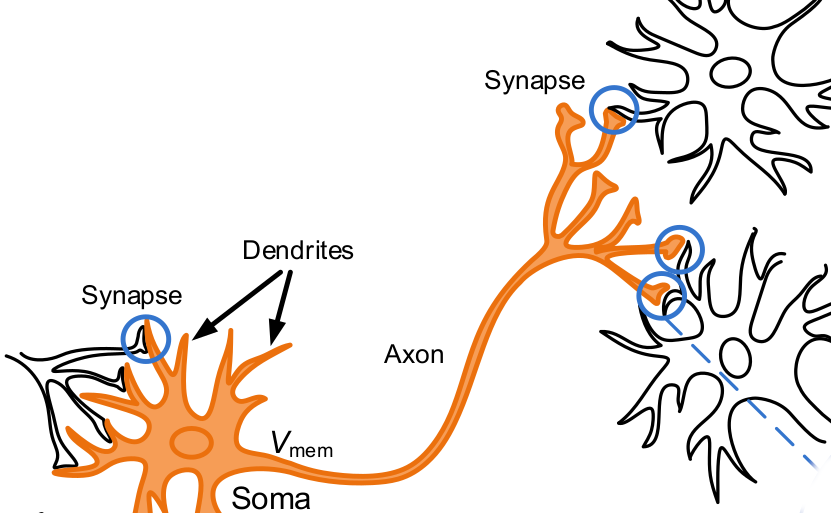
\includegraphics[scale=0.21]{neuron.png}
%%\caption{Simplified diagram of a typical biological neural cell \cite{wu2015cmos}.}
%%\label{bneuron}
%%\end{wrapfigure}
%Neuromorphic systems  include a large number of neurons, synapses and their interconnecting structure on hardware.  Such systems are highly parallel, fast, fault tolerant,  intelligent and
%compact.  This research focus is on neuromorphic systems implementing Spiking Neural Networks (SNNs). 
%Spiking neural networks  are the third generation of neural networks where neurons communicate through sparse sequences of spikes. Comparing to previous generations, SNNs
%are faster, smaller in size, more energy efficient and biologically realistic [1,2]. 
%
% Implementation of SNNs is computationally expensive because of
%nonlinear expressions in neuron models, size of the networks
%and various communication pathways.
%% A simplified  biological neuron with its corresponding connections is shown in Fig. \ref{bneuron}. A neuron could be connected to hundreds of the  other cells including neurons and astrocytes.    
% This research objective is to address this challenges by designing efficient and high speed hardware implementation platform for SNN.
%\\ [0.2cm]
%{\bf Methods: }
%%
%%One approach to study   biological neural networks is to divide it into two
%%hierarchical sub-levels of components and architecture. The
%%components level, representing the lowest level of abstraction,
%%involves studying and mathematically modeling the properties
%%and interactions of cells within the network. The architectural level,
%%however, deals with the complex interactional behaviors of
%%a large number of inter-connected components. Activities that
%%occur at the architectural level include learning and 
%%information processing in the biological neural networks. 
%%
%%At the cell level, this research has two objectives; First, is analyzing the cells  differential equation and performing bifurcation analysis  to  optimize these  ODEs for a high-performance and low-cost    implementation. Second, is designing efficient circuits for hardware implementation of these cells. These two objectives are clarified further in the following.
%%
%%
%Current neuromorphic research has led to the development of a plethora of models to mimic real neurons with different levels of abstraction in biological details [3,4]. 
%%Biologically-plausible models such as Hodgkin Huxley \cite{hodgkin1952quantitative}
%%describe cellular phenomena and properties of the individual
%%biological components. Such low-level models impose more
%%computation cost, making it difficult to simulate large-scale
%%networks. On the other hand, biologically-inspired models
%%such as Izhikevich \cite{izhikevich2003simple}, aim to
%%mimic the biological neurons to the best degree of accuracy.
%%Such models can reproduce most of the firing patterns of real
%%neurons and are easier to couple to other spike-oriented units.
%%Moreover, high-level Integrate and Fire (IF) \cite{gerstner2002spiking} is another
%%computationally efficient neuron model, but it cannot exhibit
%%many essential features of the biological neurons as observed
%%in experiments. 
%The choice of models depends
%on the application of the device to be designed. 
%%To perform
%%computations with SNNs only a simple IF or Exponential
%%IF (EIF) may be enough to act as a thresholding box.
%%However, for research in neuroscience, biologically plausible
%%models have higher flexibility in mimicking biology.
% In this research we intend to focus on
%biologically plausible and detailed models and optimize them without comprising their  correctness.  
%
% %Second objective at cell level is designing practical circuits realizing these cells using hardware implementation techniques (e.g.
%  First objective at the lowest  level is designing practical circuits realizing brain cells using hardware implementation techniques (e.g. pipelining and power optimization techniques).  It is very important to implement the cell
%models as efficient and fast as possible since they are basic building block of the neuromorphic systems. 
%Biologically plausible models are  relatively complex in nature comparing to high-level models due to their large array of differential equations and accompanying parameters.
%As a result, they have  seen limited
%proposed hardware implementations. Currently, there is no neuromorphic processor available for large scale simulation of the biologically detailed models. 
% However these models are gaining
%more attention by researchers. 
%
%
%At the architectural and software levels, brain cells are connected together through different interaction mechanisms and their systematic behavior is analyzed. 
%%T
%%his is useful to study biological functions and disorders as well as discovering computational algorithms underlying information processing, learning and memory in the brain. 
%This research has two objectives in architectural level; First is applying brain inspired learning and information processing algorithms in the software level and second is  designing a configurable hardware for large scale implementation of biological neural network. \\
%%In the following,  I will explain these two objectives in more details. 
%%
%%
%%
%%The exact mechanism of information processing and learning algorithm in the brain is yet unknown. However, 
%%Spike Timing Dependent Plasticity (STDP) is the most popular method  for unsupervised online training of 
%%feed-forward  biological neural networks. This method is based on Hebbian learning where analogous to biology, the synaptic weight changes when a pre-synaptic neuron fires
%%in a short time before or after the post-synaptic neuron,
%%strengthening or weakening the neuron connection accordingly. Such a change is determined as an exponential of the time difference between two events. 
%%
%%Large scale hardware implementation of biological neural networks could be divided into two steps. First steps is implement nonlinear bio-chemical reactions between components and second  is to design an architecture to implement  various communication pathways. 
%%\\ [0.2cm]
%{\bf Previous Research: } 
%My M.Sc. dissertation titled ``Digital Implementation of a Concise Model for Astrocyte Calcium Oscillations" was beginning of my research in the field of neuromorphic engineering where I optimized a biological astrocyte for hardware implementation using Piece Wise Linear (PWL) approximation technique. Since, I continued to research in spiking neural network and neuromorphic engineering. As a PhD student, I started using COordinate Rotation DIgital Computer (CORDIC) method to implement Izhikevch neuron and on-hardware online spike time dependent plasticity.  The advantage of CORDIC algorithm over previous methods including PWL, is its very high precision to calculate nonlinear terms and yet it is well suited for hardware implementation.  
%%In another work, a  digital implementation of a biologically plausible astrocyte and glutamate-release mechanism was presented.  
%% The designed hardware was capable of calculating nonlinear functions with a very
%%high precision while having relatively high performance. This is most important because, unlike high level models, simulation of biologically plausible models 
%%due to high biological details requires long time and computational
%%power and will fall behind the real time easily. This hardware is
%%most useful to emulate the tripartite synapse and its components.
%The primary goal of those researches was to find an appropriate hardware for neurons, astrocytes and other biological cells as buildings blocks of a biological detailed neuromorphic processor.\\
%{\bf Future Research }\\
%My future research plan involves
% both studying  algorithms underlying learning and information processing in biological neural network as well 
% designing neuromorphic processor for large scale implementation of such networks. 
%% Towards this objectives, I defined 4 projects. \\ [0.2cm]
%%{\bf Project 1} 
%%
%%This project aims  to study the different models presented by researchers to mimic biological cells that are involved in information processing in the brain. The objective is to adapt and modify differential equation describing these models to maximize performance and minimize power consumption and area. Students will run computer simulation of these models and perform bifurcation analysis to look for possible modification or approximation in these models.
%%\\ [0.2cm]
%%{\bf Project 2} 
%%
%%Designing digital circuits for ODEs describing cells. Students will use hardware implementation and optimization techniques to increase performance and reduce power consumption and area of  designs. The circuits need to be simulated to ensure their validity. 
%%\\  [0.2cm]
%%{\bf Project 3} 
%%
%%Studying interactions of the cells within the biological neural networks and investigate the mechanisms behind  learning, information processing and 
%%energy efficiency. Students will run computer simulations to observe changing of biological parameters and ions concentrations inside and around the cells that are active in learning and information processing.   
%%\\  [0.2cm]
%%{\bf Project 4} 
%%
%%Large scale implementation of the biological cells and   communication pathways in the biology. Students will design a new architecture capable of online on-chip learning with  biological neural networks. \\[0.2cm]
%%%-------------------
%%{\bf Research Program Feasibility} 
%%
%%\begin{wrapfigure}{l}{0.5\textwidth}
%%\centering
%%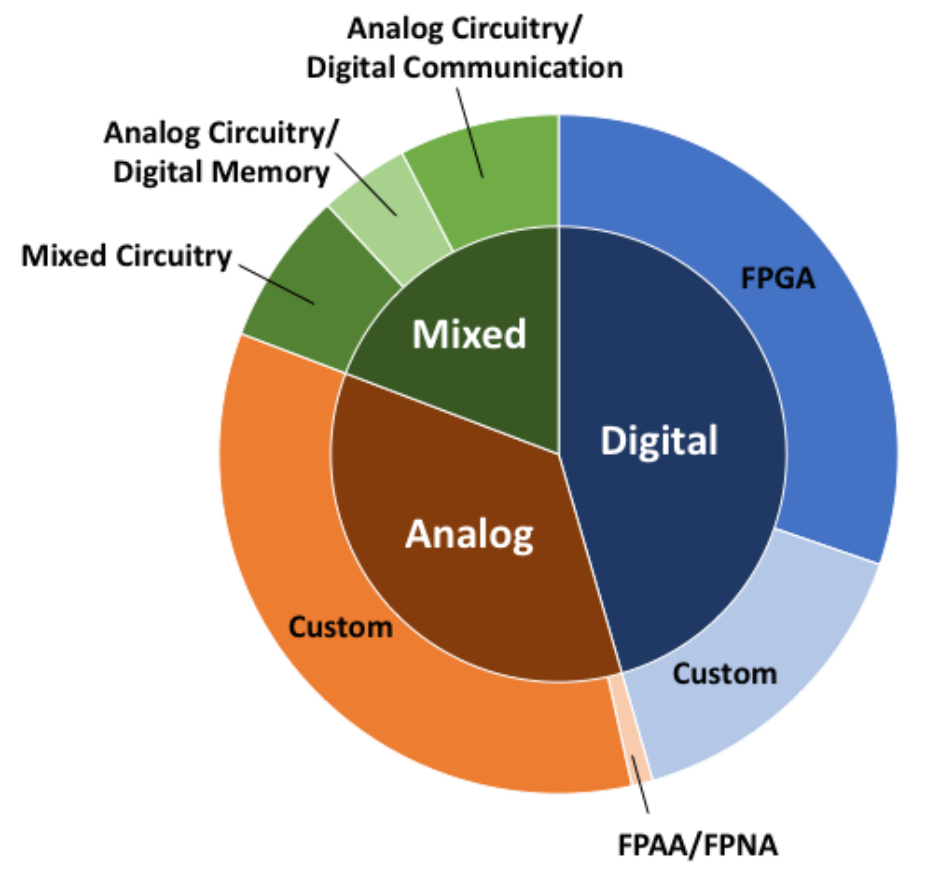
\includegraphics[scale=0.18]{hardware.png}
%%\caption{An overview of hardware implementations in neuromorphic computing \cite{schuman2017survey}.}
%%\label{fpga}
%%\end{wrapfigure}
%%The research would be initially computational, it can be  performed at a small
%%undergraduate institution. 
%Design prototypes would be implemented and tested on Field Programmable Gate Arrays (FPGAs) at first phase. FPGAs provide relatively cheap, fast, reconfigurable, and easy to work with platform for testing functionality and performance of the digital hardwares and are a popular implementation platform
% %as shown in Fig. \ref{fpga}.
%  Second phase is designing an Application Specified Integrated Circuit (ASIC)  to implement the neuromorphic processor which require softwares such Cadence that currently are accessible   through CMC Microelectronics for universities. Finally, the design need to be fabricated that is also is supported by CMC Microelectronics.
%  The primary goal of those researches was to find an appropriate hardware for neurons, astrocytes and other biological cells as buildings blocks of a biological detailed neuromorphic processor.\\
%{\bf Future Research  }\\
%My future research plan involves both studying  algorithms underlying learning and information processing in biological neural network as well designing neuromorphic processor for large scale implementation of such networks. Towards these objectives, I defined 4 projects. \\ 
%{ Project 1:} 
%This project aims  to study the different models presented by researchers . The objective is to adapt and modify differential equation describing these models to maximize performance and minimize power consumption and area. Students will run computer simulation of these models.
%{ Project 2:} Designing digital circuits for ODEs describing cells. Students will use hardware implementation and optimization techniques to increase performance and reduce power consumption and area of  designs. 
%{ Project 3:} 
%Students will run computer simulations to observe changing of biological parameters and ions concentrations inside and around the cells that are active in learning and information processing.   
%{ Project 4:} 
%Large scale implementation of the biological cells and   communication pathways in the biology. Students will design a new architecture capable of online on-chip learning with  biological neural networks. 
%{ Project 5:} software design and optimization for the hardware.
%  \\
%\hspace*{-1em}
%{\bf References} \\
%%\vspace*{-4em}
%{\footnotesize
%\phantom \quad [1] K. E. Friedl, A. R. Voelker, A. Peer, and C. Eliasmith, “Human-inspired neurorobotic system for classifying surface textures
%by touch,” IEEE Robotics and Automation Letters, vol. 1, no. 1, pp. 516–523, 2016.\\[-0.1em]
%\phantom \quad [2] F. Ponulak and A. Kasinski, "Introduction to spiking neural networks: Information processing, learning and applications.,"
%Acta neurobiologiae experimentalis, vol. 71, no. 4, pp. 409-433, 2011.\\[-0.1em]
%\phantom \quad [3] M. Samie, G. Dragffy, A. M. Tyrrell, T. Pipe, and P. Bremner, “Novel bio-inspired approach for fault-tolerant vlsi systems,”
%IEEE Transactions on Very Large Scale Integration (VLSI) Systems, vol. 21, no. 10, pp. 1878–1891, 2013.\\[-0.1em]
%\phantom \quad [4] A. L. Hodgkin and A. F. Huxley, “A quantitative description of membrane current and its application to conduction and
%excitation in nerve,” The Journal of physiology, vol. 117, no. 4, p. 500, 1952.\\[-0.1em]
%\phantom \quad [5] E. M. Izhikevich, “Simple model of spiking neurons,” IEEE Transactions on neural networks, vol. 14, no. 6, pp. 1569–1572,
%2003.
%}
%%\newpage
% \thispagestyle{empty}
% %\lhead{Research statement}
% \phantom \quad \\
%{\bf Case II: 
%Post Quantum Hardware Cryptography and Homomorphic  Encryption}\\
%%\vspace*{3\baselineskip}\\
%This research program involves reducing complexity and efficient hardware implementation of the post quantum cryptography, homomorphic encryption, and homomorphic data processing embedded systems. \\[0.2cm]
%{\bf Background:  } 
%Cryptography systems have become  inseparable parts of almost every communication device.
%Cryptography is  used to provide confidentiality, data security, and authentication in many applications such as
%communication devices, autonomous vehicles, Internet of Things (IoT), healthcare [1,2,3,4] etc.
%
%
%However, with rise of the quantum computers capable of executing Shor algorithm  [5], many popular public key cryptography systems including RSA  and elliptic curve cryptography will be no longer secure.  This would greatly endanger the security of digital communications and expose user's data. 
% National Institute of Standards and Technology (NIST) has already started a competition for developing cryptographic systems that are resistant to quantum computers attacks. At present, NIST has called for submissions for round 3 of this completion [6]. 
%%The submission for previous rounds could be find in references \citecrypto{nistr2,nistr1}. 
%
%
%Another issue with expansion of the Internet and cloud systems is privacy concern. 
% Currently, with the most secure communication between user computer and cloud system, still the data is decrypted in the cloud for processing. Therefore, the third parties owning the cloud and those with authorized access can read the data and use it for their own advantages. Homomorphic Encryption (HE), first introduced by Gentry  is a privacy preserving algorithm that allows valid computing over encrypted data without the need to decrypting it. 
% 
% Since these algorithms are expected to be the future  cryptography systems, it is important to design an efficient  embedded systems for these systems. In next section,
% I further explain my methods to address this challenge. \\
%{\bf Method: } 
%Since  post quantum cryptography is a rather new field and because of  complexity of its algorithms, there exists only a limited number of the hardware implementations for these algorithms. 
% In this research proposal, Field Programmable Gate Arrays is selected as the initial implementation target since they provide a  reconfigurable, cheap and yet fast hardware platform. 
% % Round 3  finalists for public-key encryption, key establishment and digital signature are already available in NIST website. Most of these algorithms come only with a software implementation. Even those with hardware implementation still have plenty of room for improvement. This also applies to homomorphic encryption and computation as I discuss it further in the following. 
%  In homomorphic encryption, plaintext is transformed into ciphertext, allowing computation on the encrypted data resulting in another ciphertext. Decryption of this ciphertext yields the same computation result as if it had been performed on plaintext.
% % \begin{figure}
%% \centering
%%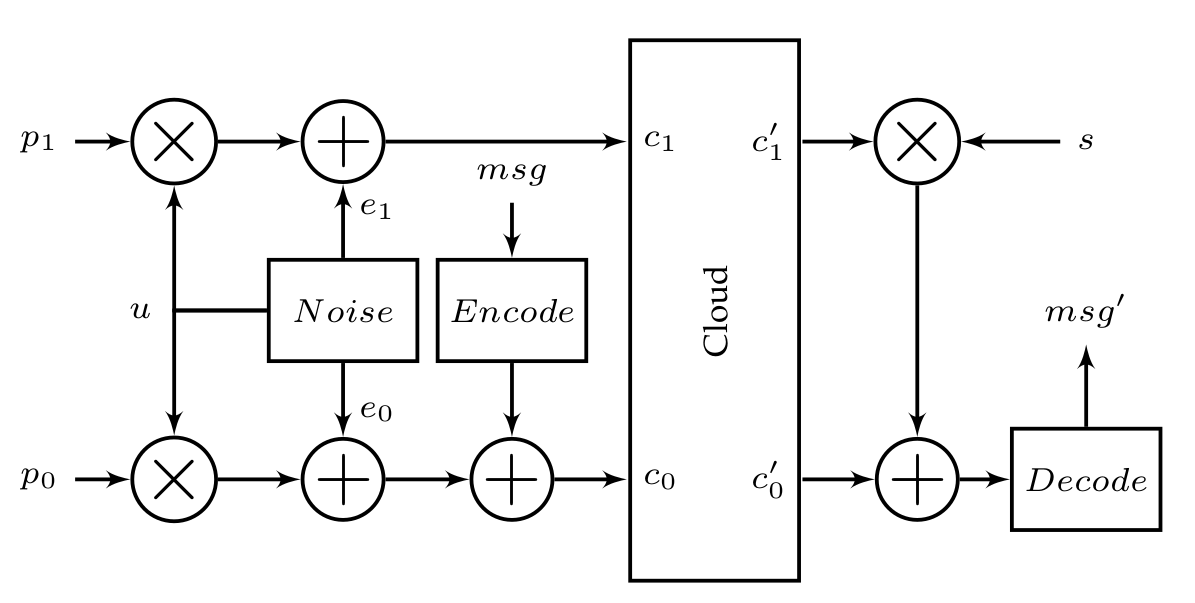
\includegraphics[scale=0.18]{fv.png}
%%  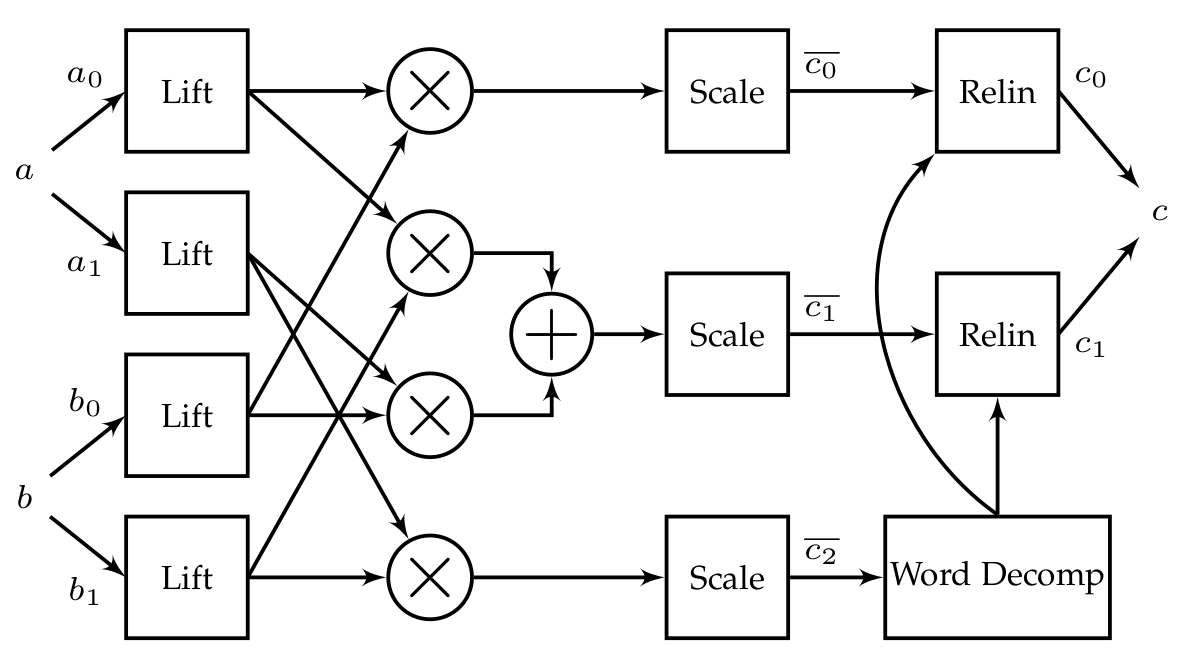
\includegraphics[scale=0.18]{fvhom.png}\\[-0.5em]
%%(a)\hspace{7.2cm}(b)
%%  \caption{(a) Fan and Vercauteren  (FV) encryption  encrypts a message into pair of ciphertexts c0 and c1 using public keys p0 and p1. 
%%  (b) Fan and Vercauteren homomorphic multiplication over the ciphertexts (figures are taken from \cite{turan2020heaws}.)}
%%  \label{hom}
%% \end{figure}
%% HE is based on lattice problems and adds noise during encryption. The value of this noise becomes greater each time an operation is performed on the ciphertext. 
%% Somewhat Homomorphic  Encryption (SHE) scheme only allows limited number of the operations on the ciphertext and more than that, the signal to noise ratio becomes so large that the original data could not be recovered anymore. Gentry in his paper introduced use of bootstrapping technique which is basically homomorphic evaluation of
%%the decryption circuit in the cloud to refresh and remove extra noises.
%% This resulted into Fully Homomorphic  Encryption (FHE). 
% However, such  operations are computationally expensive and increases the complexity of the homomorphic  computations circuit. 
%% Fig. \ref{hom} shows the circuit for homomorphic  encryption and homomorphic multiplication over encrypted data for  FV \citecrypto{fv} scheme. 
% Compared to software implementations, hardware cryptography results in a higher speed and a lower cost, while satisfying efficiency and low-power requirements of electronic
%devices. Implementation of homomorphic encryption and evaluation circuit is a extremely challenging because of the very large word length of ciphertexts and computational unit, specifically multipliers. Homomorphic encryption  is a rather new research topic and its hardware implementation is less explored. In the following, I discuss my approach towards this  problem to achieve a better hardware for practical homomorphic encryption and data processing. 
%%First, is studying the homomorphic encryption and computation to reduce their complexity and optimize them for hardware implementation. For instance, polynomial multiplication is 
%%one of  the operations that is frequently performed over very large size operands (eg. 4096 coefficients of 180-bit size  ) and plays a key role in overall performance and cost of the hardware. Therefore, it is  important to optimize these algorithm as much as possible before implementing on hardware. 
%%Second, is designing and efficient hardware architecture to encrypt and process data homomorphically. \\[0.2cm]
%\\{\bf Previous Research: }
%As postdoctoral fellow, I was working on the efficient  FPGA implementation of  finite field multipliers for Elliptic Curve Cryptography (ECC)  where we proposed a new binary polynomial multiplication algorithm with low complexity and high speed.
%The work was then extended to to hardware implementation of lattice based cryptography  algorithms and other post-quantum encryption algorithms.
%\\
%% Currently, I am closely monitoring PhD students researching in post quantum cryptography and homomorphic encryption where their research is focused on designing an FPGA based embedded processor for these algorithms.  \\
%{\bf Future Research (Research Plan): }
%My future research plan engages both studying and optimizing post quantum and homomorphic  encryption  and computation algorithms as well as designing an efficient embedded processor and processor for these algorithms. 
%%Towards this objectives, I defined 3 projects.\\[0.2cm]
%%{\bf Project 1}
%%
%%This project aims to study the different algorithms presented by researchers for 
%%post quantum cryptography including finalists of the NIST completion to standardize  quantum resistant public key cryptographic algorithms. The objective of this study is to reduce complexity and optimize these algorithms for FPGA implementation. 
%%\\[0.2cm]
%%{\bf Project 2}
%%
%%Investigating homomorphic encryption and ciphertext computation algorithms. Students will 
%%perform mathematical analysis to enhance these algorithm in the terms of area and delay complexity. Further, they will run computer simulations to check validity of the algorithms. 
%%\\[0.2cm]
%%{\bf Project 3}
%%
%%Students will design an architecture and circuit to efficiently implement  these algorithms on hardware, either as accelerator for computer software or possibly as an standalone hardware cryptography system.\\[0.2cm]
%\\{\bf Research Program Feasibility: }
%For the first phase which is optimizing  algorithms for hardware implementation, I will use Python programming language to run simulations and check the validity of  modified algorithms.  Further, I will use FPGAs as implementation platform to measure efficiency of design. FPGAs are substantially cheaper than designing  and fabricating a VLSI ASIC and have advantage of flexibility. Eventually, after testing design could be fabricated for final evaluations. Towards this objectives, I defined 3 projects:
% Project 1: 
%This project aims to study the different algorithms presented by researchers for 
%post quantum cryptography including finalists of the NIST completion to standardize  quantum resistant public key cryptographic algorithms. The objective of this study is to reduce complexity and optimize these algorithms for FPGA implementation. 
%{ Project 2:}
%Investigating homomorphic encryption and ciphertext computation algorithms. Students will 
%perform mathematical analysis to enhance these algorithm in the terms of area and delay complexity. Further, they will run computer simulations to check validity of the algorithms. 
%{ Project 3:}
%Students will design an architecture and circuit to efficiently implement  these algorithms on hardware, either as accelerator for computer software or possibly as an standalone hardware cryptography system.
%\\{\bf Funding for research }
%In terms of funding , I would be able to use my background and familiarity with problems and concerns of industry to secure funding for the research. I have also experience of writing successful research proposal with industry partner to obtain MITACS grant. \\ 
%\hspace*{-1.8em}
%{\bf References} \\
%%\vspace*{-4em}
%{\footnotesize
%\phantom \quad [1] J. Yoo and J. H. Yi, “Code-based authentication scheme for lightweight integrity checking of smart vehicles,” IEEE Access,
%vol. 6, pp. 46731–46741, 2018.\\[-0.1em]
%\phantom \quad [2] R. Abu-Salma, M. A. Sasse, J. Bonneau, A. Danilova, A. Naiakshina, and M. Smith, “Obstacles to the adoption of secure
%communication tools,” in 2017 IEEE Symposium on Security and Privacy (SP), pp. 137–153, 2017.\\[-0.1em]
%\phantom \quad [3] P. Aparna and P. V. V. Kishore, “Biometric-based efficient medical image watermarking in e-healthcare application,” IET
%Image Processing, vol. 13, no. 3, pp. 421–428, 2019.\\[-0.1em]
%\phantom \quad [4] T. D. P. Bai, K. M. Raj, and S. A. Rabara, “Elliptic curve cryptography based security framework for internet of things (iot)
%enabled smart card,” in 2017 World Congress on Computing and Communication Technologies (WCCCT), pp. 43–46, 2017.\\[-0.1em]
%\phantom \quad [5] P. W. Shor, "Algorithms for quantum computation: discrete logarithms and factoring," Proceedings 35th Annual Symposium on Foundations of Computer Science, 1994, pp. 124-134, doi: 10.1109/SFCS.1994.365700\\[-0.1em]
%\phantom \quad [6] “Post-Quantum Cryptography-Round 3 Submissions,” 2020.
%
%}
%\newpage
% \thispagestyle{empty}
% \lhead{Teaching Statement}
% \phantom \quad \\
% {\bf Teaching Statement}
\vspace*{3\baselineskip}\\
{\bf Inspiration}

My father was a teacher. He always inspired me to learn by asking questions and intriguing my sense of curiosity. The same sense of curiosity  that grew my motivation to continue  my education and become a researcher. One quality that I most like about him and later, became a part of my character as well, was his critical way of thinking and teaching.  Instead of giving direct answers to my questions, he guided me and encouraged me to discover the answers for myself.
 From what I learned, it is the disciplined practice of critical thinking that
enables  students to examine ideas, determine their validity and become creative.  
In short,  a great teacher provides students with the motivation toward becoming a knowledgeable and innovative person.
My approach to teaching
 is based on same idea of critical thinking and has three main components: Inquiry,  a deep understanding, and novelty.
 \\ [0.2cm]
{\bf Inquiry }

I believe that the best way  to encourage students is inquiry-based learning. 
Students tendency toward a new concept will be higher when they believe that it can be answer to a problem in their minds.  
The idea is to start the class with a few well-chosen questions and have the students explore the topic themselves, with guidance from the teacher. 
In this method, I will express the fundamental problem,
 encourage my students with a desire to know the answer and then  let the class  discusses it. 
 My role would be more an moderator who leads students in a challenging experience  planned to promote discussion, thinking and discovery. As an example,  when I started Digital Logic Design at  beginning of the semester and intended to talk about number systems,  I initiated the class with the questions  "why predominant number system is decimal and why not for instance, octal or hexadecimal?"
 And after discussing that, I asked the next question "now, why machines use binary number system?".  I observed that larger number of students engaged in answering the second question, when the first question was discussed in advance, compared to classes when I went directly for the second questions. 

%As an example, I when I started Digital Logic Design at  beginning of the semester and intended to talk about number systems,  I initiated class with the question  "why the predominant number system is decimal and why not for instance, octal or hexadecimal?"
%I observed that these question intrigues students sense of curiosity.
% And after that I asked another question "why machines use binary number system?".
% I observed that number of  students  participate in the class  answering this question increase when the first question asked before this. 

 
 
 This method also leads to conceptual understanding of the the problems and solutions in electrical engineering.    
   Students with conceptual understanding know more than solitary facts and methods and are able to  connect different concepts, decipher problems,  and apply engineering methods in novel ways. \\[0.2cm]
   {\bf A Deep Understanding}
   
   A good teaching method is a combination of different  techniques. Another technique that I find to be most useful is  cognitive learning where learning focus is on understating the 
subject at the deeper level rather than memorization of approaches toward certain problems.
  My approach toward this process is based on the following elements:  First, students need to understand why they are learning the subject. Second, is gaining knowledge about the subject at a deep level and third, is to contemplate on the application of what they learned. 
 The course contents need to be designed in a way that the students get a deep understanding  and develop the skills to apply their knowledge in their field. 
    
    An example is when I was presenting logical operations (AND, OR and NOT) at a Digital Logic Design class. First, I explained the concept of idealized switches network 
    where switches are considered as having only two exclusive states of open or close. Further, I gave them simple examples and  asked them    to identify different combinations and make separate components.      Later, I  introduced the Boolean algebra and logical
operations as a way to analyze and design circuits by algebraic means in terms of logic gates. \\[0.2cm]
   {\bf Creativity}
   
Perhaps the most important part of learning  and at the highest level, is creativity. 
    The scientific approach toward creativity involves studying  and mastering what have been achieved so far, asking  questions, proposing  solutions, designing experiments to check validity of the solutions and finally communicating the research with other scientists to have feedbacks. 
    
    My plan to engage graduate  and last year undergraduate students in research would be by means of the following. First, I will give them enough background and knowledge in a specific area which I believe have potential for research. Further, I will ask them to identify and make a list of the new and prominent works published in the subject. Afterwards, I will ask them to write a short brief on those papers and identify  their contributions. The next step would be presentation of the papers that foster deeper understanding of the works. Personally, I believe explaining something to someone else helps to have better insight about the topic.  Therefore, such conferences would be an fundamental part of my approach which  helps students both to evaluate the literature and communicating their findings.    
    
    The next move would be critical analysis of the papers. Students need to think about the weaknesses, limitations and drawbacks of the proposed approaches. Performing simulations in order to   replicating and testing findings on the papers also helps them to 
    learn the required tools and approaches toward the problems and also facilitate spotting the problems.
    
    At end of any phase, it is my duty as a teacher to evaluate their work and give them feedbacks and suggestions to improve their work. This will give students the opportunity to improve their ability to identify the problem, review the literature  for solutions, propose new solutions and finally communicating their research. 
    
    
    In summary, I wish to give back those qualities that meant the most to me during my
education: inquiry, a deep understanding and creativity. I hope to develop the love of engineering in my students since personally, I feel an infinite passion for it. As a saying states: "Choose a career you love and you will never have to work a day in your life".

%\newpage
% \thispagestyle{empty}
% \lhead{Diversity Statement}
% \phantom \quad \\
% {\bf Diversity Statement}
%\vspace*{3\baselineskip}\\
%
%
%
%I was born in Iran,  in a city close to Iraq border, during the long and bloody war between Iran and Iraq. My parents had to leave everything behind and flee to  safer zones several  times. When I was three years old, there was a ceasefire and war was finally over after eight years. I don't remember much about the war; However, I could clearly feel and see the aftermath. There were people who lost their loved ones and were always sad, some lost a limb and became disabled, many suffered mental problems and most people, including our family, lost their home and all possessions because of bombings. This war, that left more than one million casualties and losses, was mainly over religious difference. I 
%deeply sensed and suffered from consequences of a flare up religious hate, and  as a child,  promised myself that never let hatred grow in my heart and I do everything I can to help people tolerate and understand each other. 
%
%
%Like many, we lost our home during aerial bombardments. My father was a teacher and we were fortunate to have a source of income.  Still, economy of the country was devastated after the war. My father  could only afford to build a room in ruins of our house and there was no electricity or running water.   Stealing and street violence crimes started to increase   in a way that my father  had to walk me to school before going to his work. 
% It was not uncommon for my neighborhood friends to have a drug abusing parent, a single parent household,  or experience domestic violence.   Living under such circumstances were   difficult but it gave me a valuable experience and I  can still fully understand  how it feels to be financially insecure and live in a dangerous neighborhood. 
%
%
%
%
%Later in school, I faced yet another challenge. Our city was a Kurdish region and I used to speak Kurdish with my family, friends and everyone else. However, the official language in the school and all textbooks were in Persian. Speaking Kurdish was forbidden in school and It was very difficult for me as child to suddenly start reading, writing and speaking a new language. I became fluent in the language, but moving out to other cities to continue education and subsequently finding a job where I faced more and more discrimination and
%humiliation because of my background. 
%
% As results of such systematic racism and being culturally oppressed, many people were ashamed to talk their mother tongue and begin to hide their ethnicity.  To fight this, I started a blog and developed android applications  to rise awareness that everyone has the right to speak their mother tongue and no body should ever be shamed of his race or background. My experience as a member of an
%ethnic minority has greatly helped me to better understand others who face similar
%challenges based on their identity.
%
%
%
%
%
%
%
%My commitment to promoting diversity and inclusion in academia is grounded in my personal experience. During my PhD in Canada, I was fortunate to work alongside insightful faculty members in University of Windsor. I was truly inspired by their commitment to social justice, diversity and inclusion. I became friends with people from  LGBTQ community.  Hearing their stories and experiences, and learning that some are still afraid to come out and be honest about their identity, reminded of my own experience as an ethnic minority. 
% I truly admired them and hope that one day no one experience stigma and discrimination because of sexual orientation. 
%  I have had the opportunity to address diversity and inclusion  in my roles as Graduate Assistant and Postdoctoral Fellow at University of Windsor. 
% I am committed to create an environment free from discrimination based on the race, religion, sex, economic status, sexual orientation, disability or other characteristics.
% 

\end{document}
